\documentclass[sans,
%compress,% maximize space for content
frameno, % add frame counter
%splitnav,
mp,
usenames,dvipsnames, % colors
onlytextwidth, %columns with the same textwidth as the par text
t,%align on top by default
11pt]{beamer}
% \usefonttheme{serif}
\usepackage{opencolor}
\usepackage[version=4]{mhchem}
\usepackage{siunitx}
\usetheme{Arguelles}
\usepackage[labelfont=bf, skip=2pt, figureposition=bottom, font=footnotesize, textfont=it]{caption}
\captionsetup[figure]{labelformat=empty}
%\captionsetup[table]{labelformat=empty}
\captionsetup{belowskip=-8pt}
\usepackage{tikz}
\usepackage[export]{adjustbox}
\usepackage{multirow}

%% custom commands
\newcommand{\notice}[1]{\textbf{\alert{#1}}}
\newcommand{\iso}[2]{\ce{^{#1}#2}}


%% Modify beamer templates
\setbeamertemplate{caption}[numbered]
%\setbeamerfont{caption name}{series=\bfseries}
%\setbeamertemplate{caption label separator}[period]


%\title{$(d, \iso{3}{He})$ transfer reactions}
\title{Transfer reactions with Be-Li isotopes near the drip-line}
\event{LISE Workshop 2024}
\date{\empty}
\author{M. Lozano-González, A. Matta, B. Fernández-Domínguez, 
\texorpdfstring{\\}{} J. Lois-Fuentes, F. Delaunay \texorpdfstring{\\}{}
{\small on behalf on the E748 collaboration}}
\institute{IGFAE\textminus USC and LPC\textminus Caen}

\begin{document}

\frame[plain]{\titlepage}

%\stretchon
\Section{Motivation}
\begin{frame}[t]{Overview of the exotic Be-Li region}
    Be and Li isotopes close to the neutron drip line have been extensively studied due to their exotic properties.

    Two prime examples can be showcased:

    \medskip
    \begin{columns}[c]
        \only<+>
        {
            \column{0.48\linewidth}
            {
                \noindent\notice{\iso{11}{Li}} is a neutron-rich nuclei displaying a 2n \textbf{halo} structure.

                \bigskip

                \bigskip
                \begin{figure}
                    \centering
                    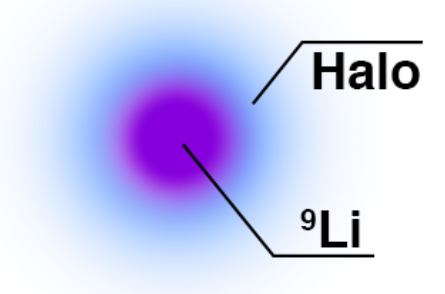
\includegraphics[width=0.7\linewidth]{figures/11Li.png}
                \end{figure}
            }
            \hfill
            \column{0.5\linewidth}
            {
                \begin{figure}
                    \centering
                    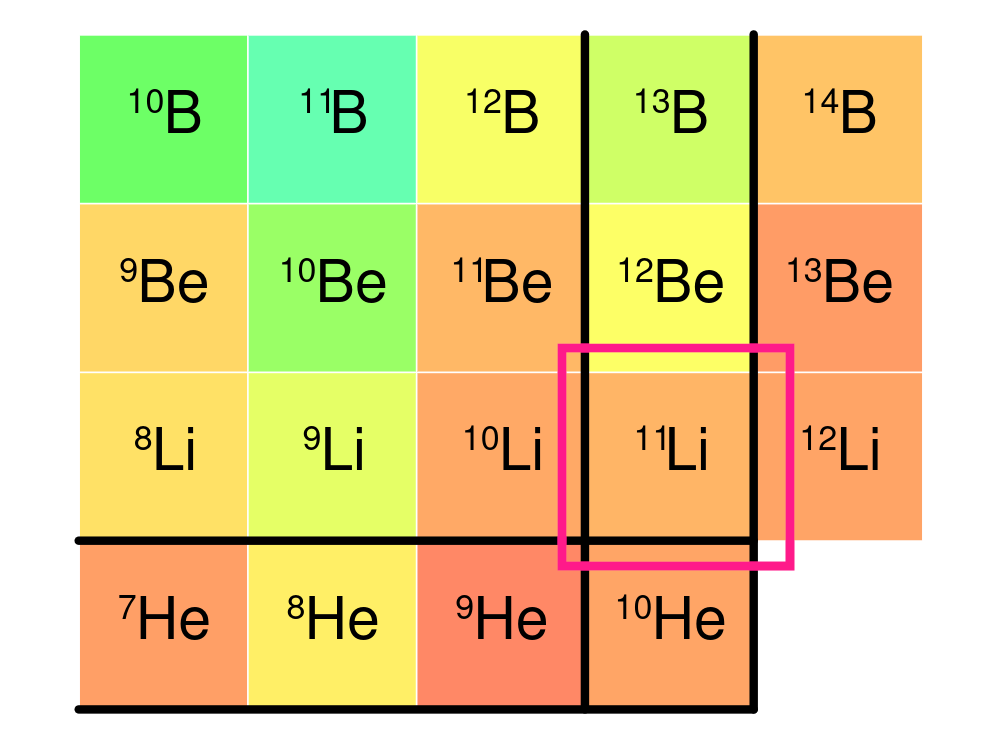
\includegraphics[width=0.9\linewidth]{figures/chart_new_11Li.png}
                \end{figure}
            }
        }
        \only<+>
        {
            \addtocounter{framenumber}{1}
            \column{0.48\linewidth}
            {
                \notice{\iso{11}{Be}} presents parity inversion: g.s has \textbf{positive} parity when negative expected.
                \bigskip
                \begin{figure}
                    \centering
                    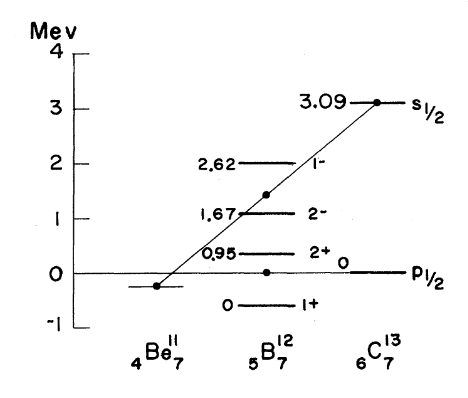
\includegraphics[width=0.75\linewidth]{figures/11Be_paper.png}
                    \caption{I. Talmi and I. Unna, PRL 4 (1960).}
                \end{figure}
            }
            \hfill
            \column{0.5\linewidth}
            {
                \begin{figure}
                    \centering
                    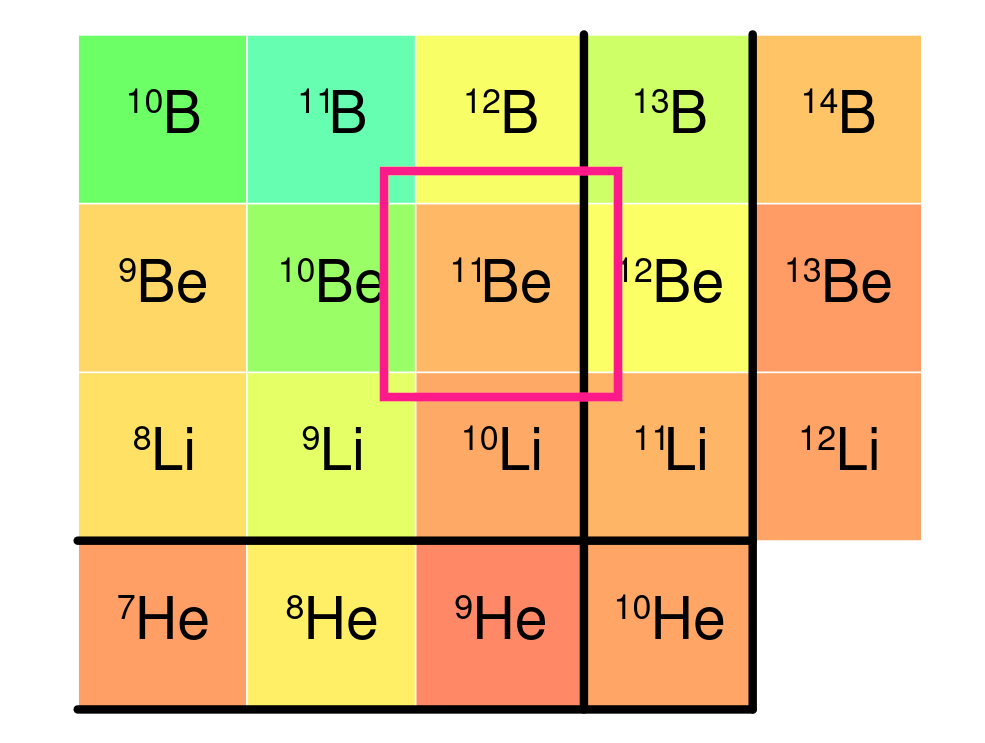
\includegraphics[width=0.9\linewidth]{figures/chart_new_11Be.png}
                \end{figure}
            }
        }
    \end{columns}
\end{frame}

\begin{frame}[t]{Recently gathered information}
    During the MUST2 @ RIKEN campaign, an unexpected \textbf{reduction} of the cross-section was observed in $\iso{9,11}{Li}(\textrm{d}, \iso{3}{He})\iso{8,10}{He}$ reactions.
    \begin{figure}
        \centering
        \includegraphics<1>[width=0.7\linewidth]{figures/matta_experiment.png}
        \includegraphics<2>[width=0.8\linewidth]{figures/wf_12Be.pdf}
        \caption{\only<1>{A. Matta et al., PRC 92 (2015).}
            \only<2>{GMF of neutron w.f for \iso{12}{Be}(d, \iso{3}{He})\iso{11}{Li}}}
    \end{figure}

    \bigskip
    \begin{columns}
        \column{0.68\linewidth}
        {
            Possible \notice{explanations}:
            \begin{itemize}
                \item<1,2> Role of the many-body interactions.

                \item<2> Overestimation of the nuclear overlap $\left\langle \iso{9,11}{Li} \middle| \iso{8,10}{He}\right\rangle$.

            \end{itemize}
        }
        \hfill
        \column{0.3\linewidth}
        {
            \only<2>{
                \begin{beamercolorbox}[sep=1.25ex,center, rounded=true]{boxgreenish}
                    \textbf{Collect} more $\textrm{d}\sigma / \textrm{d}\Omega$ data!
                \end{beamercolorbox}
            }
        }
    \end{columns}
\end{frame}

\Section{Methodology}
\begin{frame}{Reactions to be studied}
    \textbf{E748} at GANIL during the MUST2@LISE campaign. Neutron and proton removal reactions from \iso{10,12}{Be} beams have been performed to probe key nuclei:

    \bigskip
    % \begin{columns}
    %     \column{0.45\linewidth}
    %     {
    %         \begin{itemize}
    %             \item<1,2,3,4> \textbf<1>{\iso{10}{Be}(d, t)\iso{9}{Be}}: Benchmark reaction. n-\textbf{occupancy} in $p_{3/2}$.

    %             \item<2,3,4> \textbf<2>{\iso{10}{Be}(d, \iso{3}{He})\iso{9}{Li}}: $p_{3/2}$ proved but on the proton side.

    %             \item<3,4> \textbf<3>{\iso{12}{Be}(d, t)\iso{11}{Be}}: higher orbital $p_{1/2}$.

    %             \item<4> \textbf<4>{\iso{12}{Be}(d, \iso{3}{He})\iso{11}{Li}}: same p-orbital as before.
    %         \end{itemize}
    %     }
    %     \hfill
    %     \column{0.5\linewidth}
    %     {
    %         \only<1>{\begin{figure}
    %                 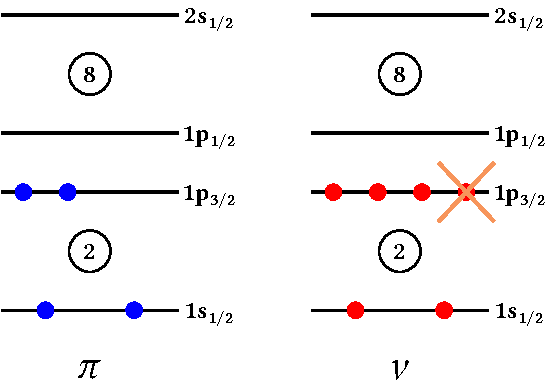
\includegraphics[width=\linewidth]{figures/shell_model_9Be.pdf}
    %                 \caption{\textbf{\iso{10}{Be}} shell model.}
    %             \end{figure}
    %         }
    %         \only<2>{\begin{figure}
    %                 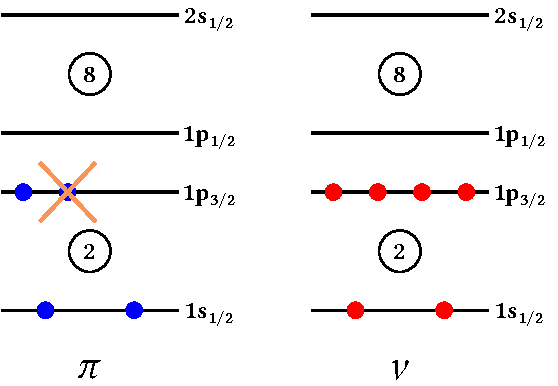
\includegraphics[width=\linewidth]{figures/shell_model_Lis.pdf}
    %                 \caption{\textbf{\iso{10}{Be}} shell model.}
    %             \end{figure}
    %         }
    %         \only<3>{\begin{figure}
    %                 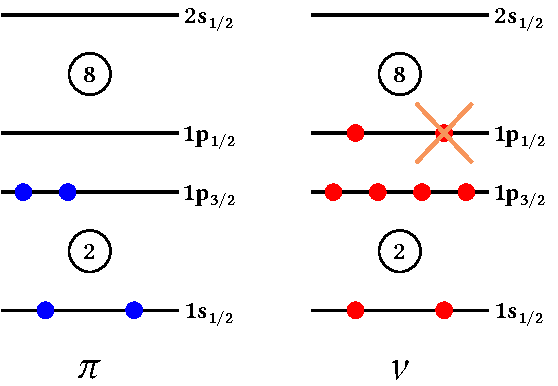
\includegraphics[width=\linewidth]{figures/shell_model_11Be.pdf}
    %                 \caption{\textbf{\iso{12}{Be}} shell model.}
    %             \end{figure}
    %         }
    %         \only<4>{\begin{figure}
    %                 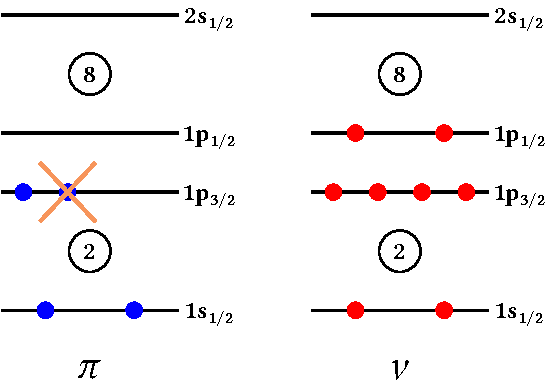
\includegraphics[width=\linewidth]{figures/shell_model_11Li.pdf}
    %                 \caption{\textbf{\iso{12}{Be}} shell model.}
    %             \end{figure}
    %         }
    %     }
    % \end{columns}
    \begin{figure}
        \centering
        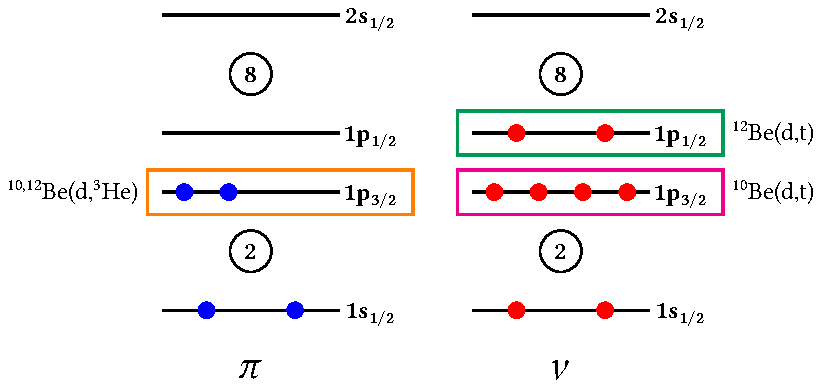
\includegraphics[width=0.7\linewidth]{figures/Workshop/shell_model_all.pdf}
        \caption{Shell model for \iso{10,12}{Be}}
    \end{figure}
\end{frame}

\begin{frame}{Experimental setup for E748}
    Traditional \textbf{solid target} experiment @ D6. Below a sketch of the setup:

    \begin{figure}
        \centering
        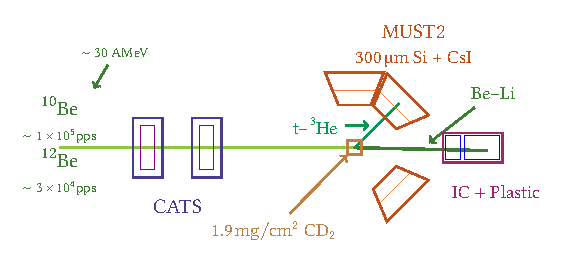
\includegraphics[width=\linewidth]{figures/setup.pdf}
    \end{figure}
\end{frame}

\begin{frame}{Analysis at a glance}
    A \textbf{common} procedure is employed in all the reactions. Different gates are applied in a sequential manner, as follows:

    \bigskip
    \only<1>
    {
        \begin{columns}[c]
            \column{0.5\linewidth}
            {
                \begin{enumerate}
                    \item[1.] \textbf{Heavy ID}: Only distinction in $Z$: separation of Be from Li residuals, but not along isotopic chain.
                \end{enumerate}
            }\hfill
            \column{0.45\linewidth}
            {
                \begin{figure}
                    \centering
                    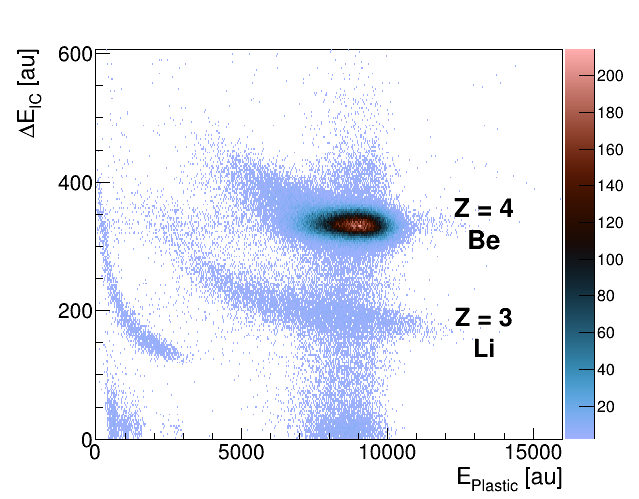
\includegraphics[width=1\linewidth]{figures/Workshop/heavy.png}
                \end{figure}
            }
        \end{columns}
    }
    \only<2>
    {
        \addtocounter{framenumber}{1}
        \begin{columns}[c]
            \column{0.5\linewidth}
            {
                \begin{enumerate}
                    \item[2.] \textbf{Light ID}: Using only stopped particles in Si layer, but low TOF resolution. Separation of \notice{\textbf{t \textminus \iso{3}{He}}} attained with kinematics!
                        % \item[3.] We are ready to compute $\mathbf{E_{x}}$ with the \textbf{missing mass technique}!  
                \end{enumerate}

                \bigskip

                \begin{center}
                    \begin{beamercolorbox}[sep=1.25ex,center, rounded=true, wd=0.9\linewidth]{boxmyviolet}
                        Missing mass technique: \\
                        $E_{\textrm{beam}} + (E,\theta)_{\textrm{Lab}} \rightarrow \mathbf{E_{x}}$
                    \end{beamercolorbox}
                \end{center}
            }\hfill
            \column{0.45\linewidth}
            {
                \addtocounter{figure}{1}
                \begin{figure}
                    \centering
                    \includegraphics<2>[width=1\linewidth]{figures/Workshop/light.png}%
                    % \includegraphics<3>[width=1\linewidth]{figures/tof_pid.png}
                \end{figure}
            }
        \end{columns}
    }

\end{frame}

\Section{Results}
\begin{frame}{Elastic: $\iso{10}{Be}(\textrm{d}, \textrm{d})\iso{10}{Be}$}
    \only<+>{
        Serves as a test of the analysis, allowing us to ascertain the \textbf{normalization} factors $N_t$ and $N_b$.
        \begin{figure}
            \begin{minipage}[t]{0.48\linewidth}
                \centering
                \begin{tikzpicture}
                    \node[anchor=south west,inner sep=0] (image) at (0,0) {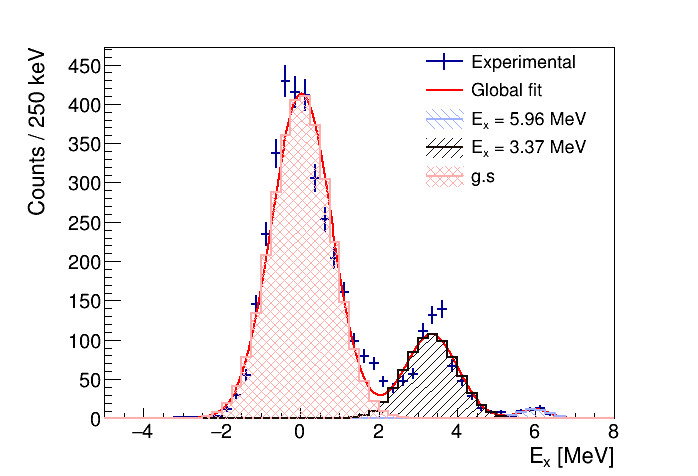
\includegraphics[width=\textwidth]{figures/Workshop/10Be_dd_ex.png}};
                    \begin{scope}[x={(image.south east)},y={(image.north west)}]
                        % \draw[step=0.05,gray,very thin] (0,0) grid (1, 1);
                        \draw[->, very thick, VioletRed] (0.42,0.99) -- (0.42,0.88);
                    \end{scope}
                \end{tikzpicture}
            \end{minipage}
            \hfill
            \begin{minipage}[t]{0.48\linewidth}
                \centering
                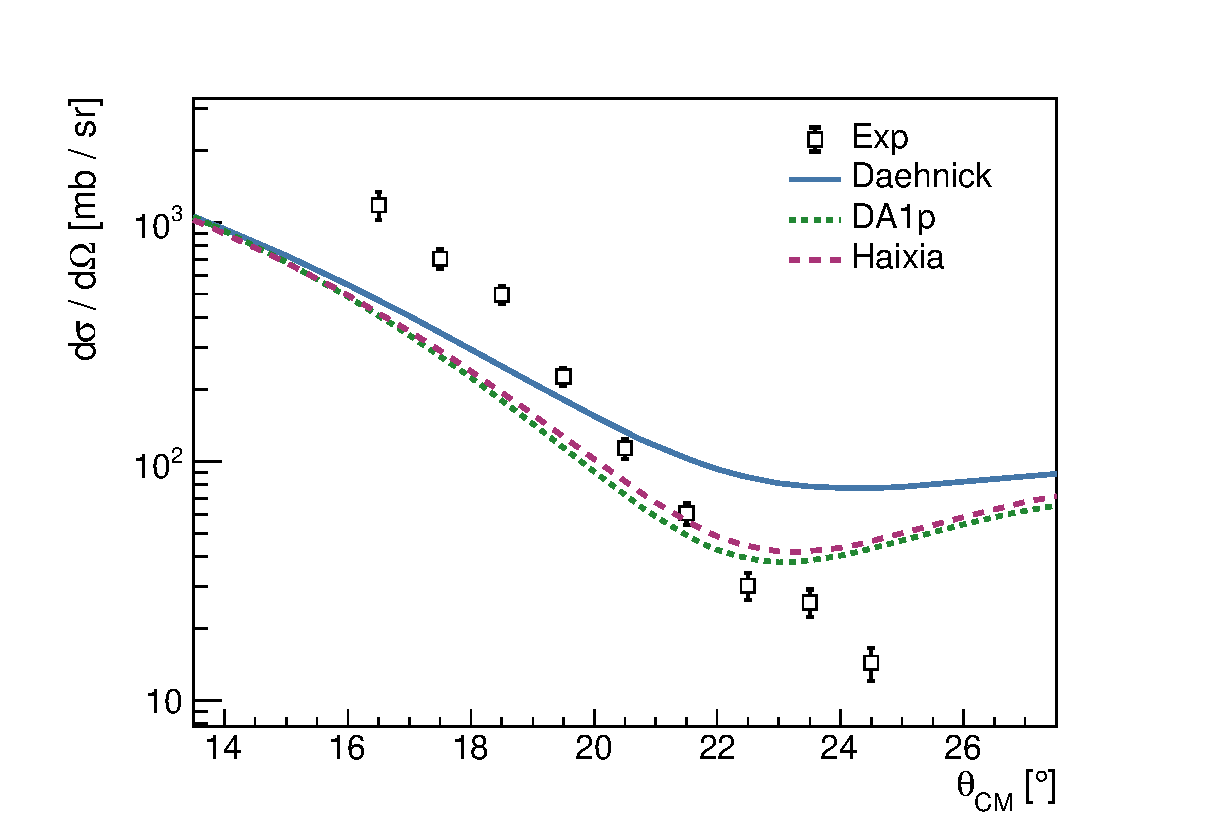
\includegraphics[width=\textwidth]{figures/Workshop/10Be_dd_xs.eps}
            \end{minipage}
        \end{figure}
        \begin{columns}
            \column{0.58\linewidth}
            {
                \begin{itemize}
                    \item Modern models (Haixia and DA1p) adjust better the minimum.
                          % \item Failure at low and high angles.
                    \item Overall agreement in magnitude.
                \end{itemize}
            }\hfill
            \column{0.38\linewidth}
            {

                \begin{beamercolorbox}[sep=1ex, center, rounded=true]{boxmyorange}
                    Error in \textbf{efficiency} \\
                    \medskip
                    Proton \textbf{contamination} at low $E$
                    % Likely to be a miscalculation in \textbf{efficiency}
                \end{beamercolorbox}

            }
        \end{columns}
    }
    \only<+>{
        Cross-section for the 1st excited state is also achievable.
        \begin{figure}
            \begin{minipage}[t]{0.48\linewidth}
                \centering
                \begin{tikzpicture}
                    \node[anchor=south west,inner sep=0] (image) at (0,0) {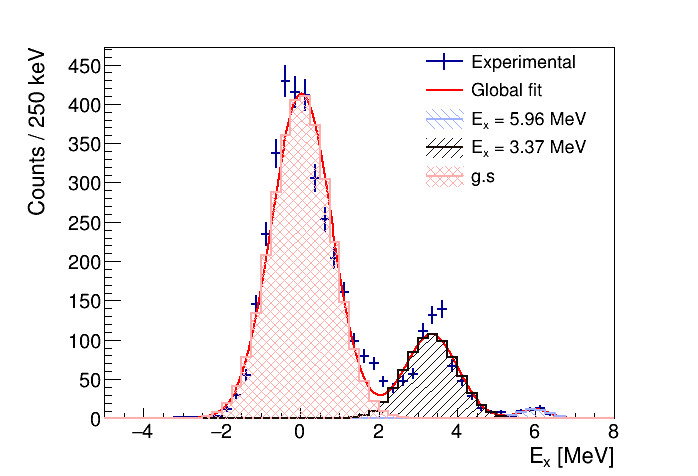
\includegraphics[width=\textwidth]{figures/Workshop/10Be_dd_ex.png}};
                    \begin{scope}[x={(image.south east)},y={(image.north west)}]
                        % \draw[step=0.05,gray,very thin] (0,0) grid (1, 1);
                        \draw[->, very thick, VioletRed] (0.61,0.55) -- (0.61,0.39);
                    \end{scope}
                \end{tikzpicture}
            \end{minipage}
            \hfill
            \begin{minipage}[t]{0.48\linewidth}
                \centering
                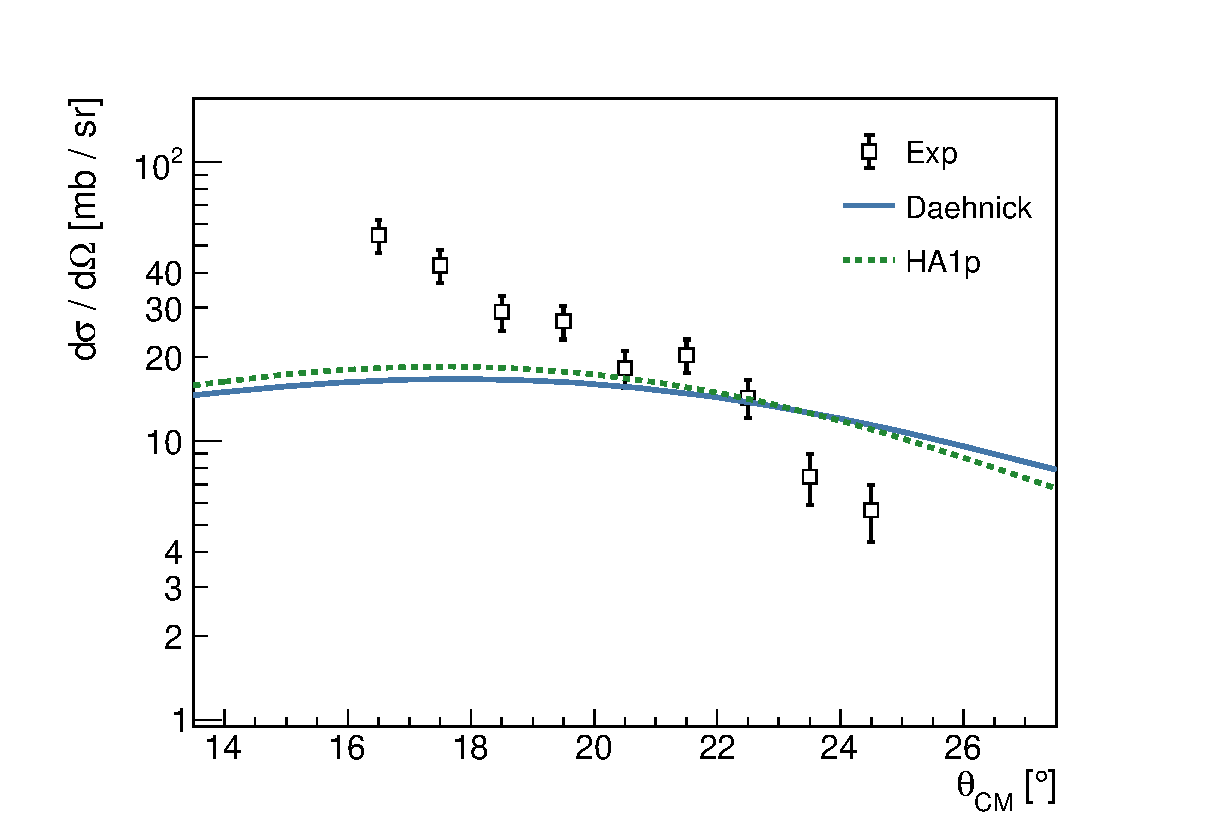
\includegraphics[width=\textwidth]{figures/Workshop/10Be_dd_xs_g1.eps}
            \end{minipage}
        \end{figure}
        \begin{columns}
            \column{0.58\linewidth}
            {
                \begin{itemize}
                    \item DWBA: potential deformed in both Coulomb and nuclear parts
                    \item Using $B(E2)$ from other experiments
                    \item \notice{Same} error as before?
                \end{itemize}
            }\hfill
            \column{0.38\linewidth}
            {

                \begin{beamercolorbox}[sep=1ex, center, rounded=true]{boxmyorange}
                    To be further investigated. \\
                    $\Rightarrow C^2S = \qty{0.270(22)}{}$ with Daehnick
                \end{beamercolorbox}

            }
        \end{columns}
    }
\end{frame}

\begin{frame}{Neutron removal: $\iso{10}{Be}(\textrm{d}, \textrm{t})\iso{9}{Be}$}
    \only<+>
    {
        Only the \textbf{ground state} is accessible. Angular distributions are determined in the interval $\theta_{\textrm{CM}} \in \left[5, 20\right]\unit{\degree}$.
        \begin{figure}
            \begin{minipage}[t]{0.48\linewidth}
                \centering
                \begin{tikzpicture}
                    \node[anchor=south west,inner sep=0] (image) at (0,0) {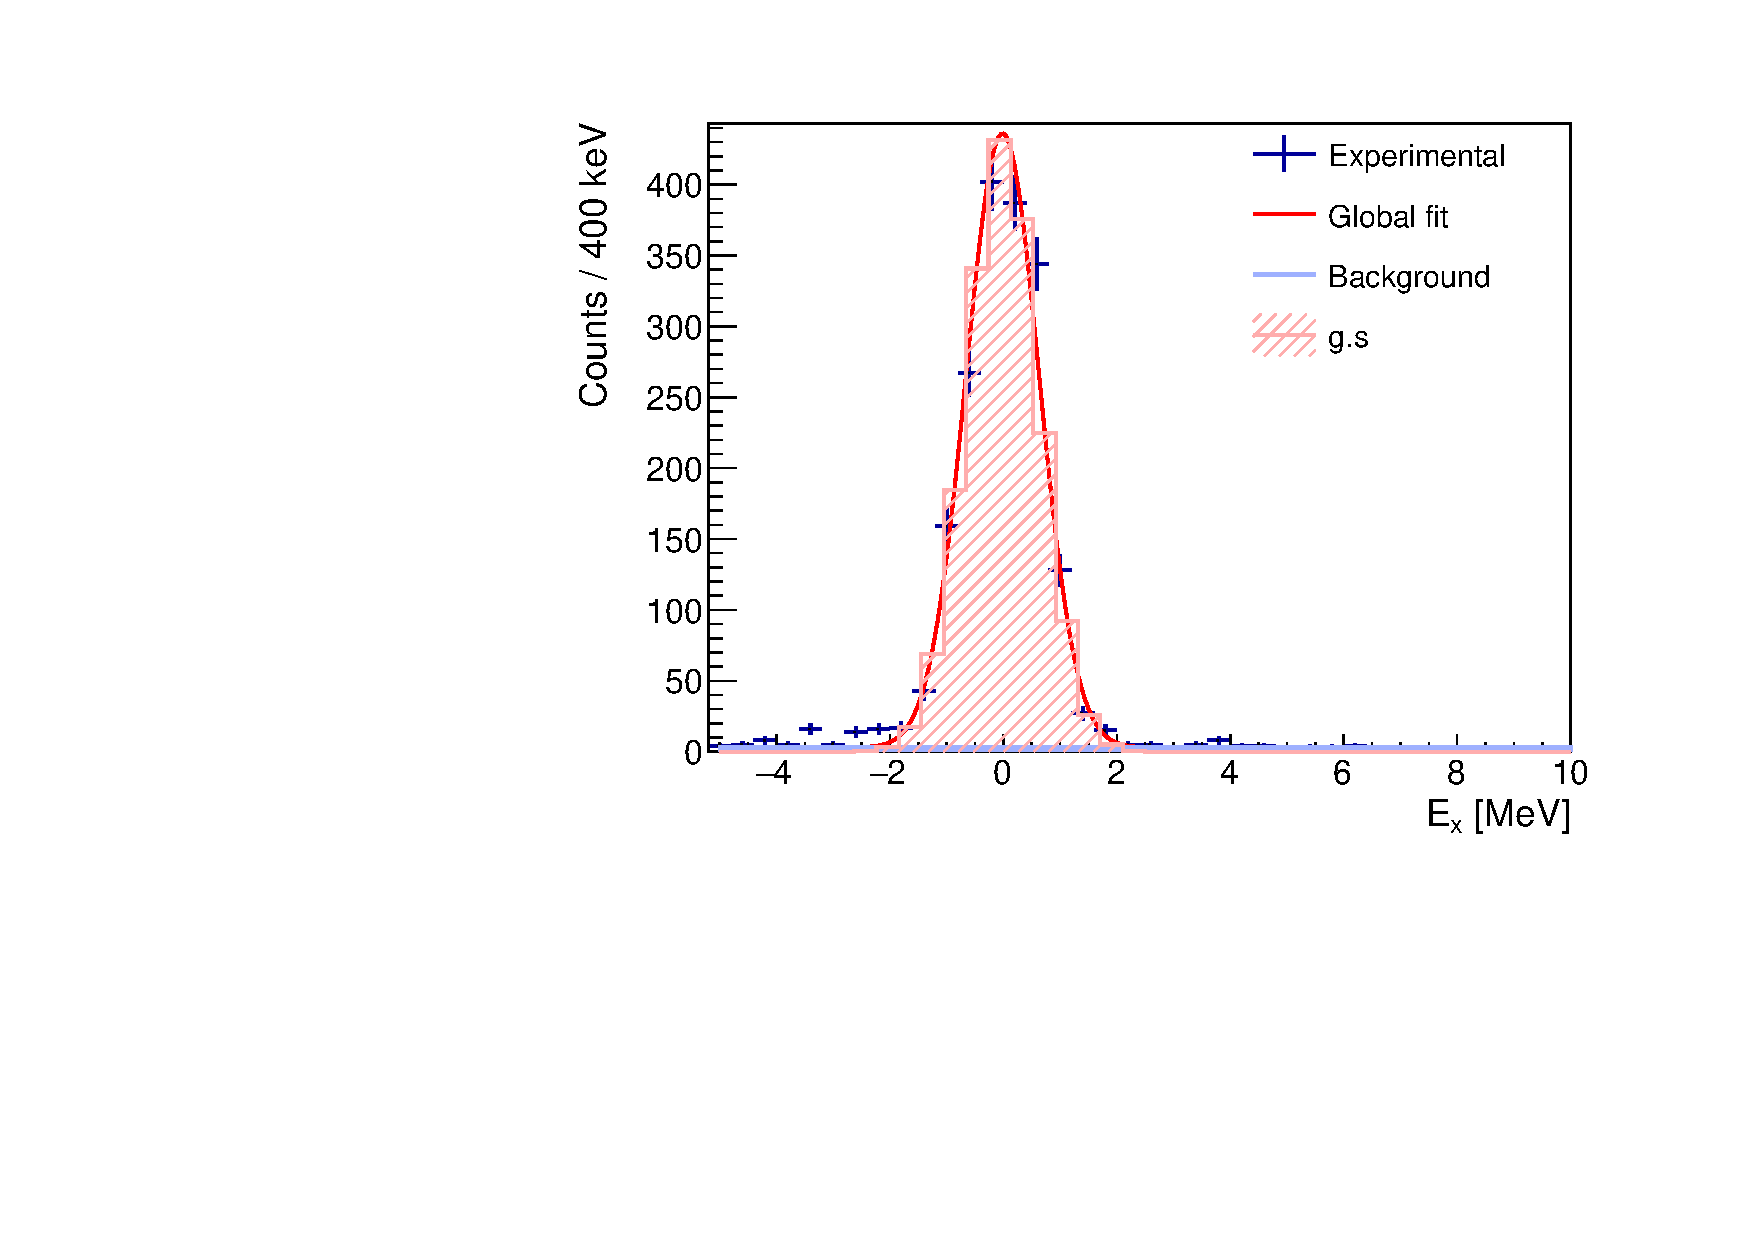
\includegraphics[width=\textwidth]{figures/Workshop/10Be_dt_ex.pdf}};
                    \begin{scope}[x={(image.south east)},y={(image.north west)}]
                        %\draw[step=0.05,gray,very thin] (0,0) grid (1, 1);
                        \draw[->, very thick, VioletRed] (0.40,0.99) -- (0.40,0.90);
                    \end{scope}
                \end{tikzpicture}
            \end{minipage}
            \hfill
            \begin{minipage}[t]{0.48\linewidth}
                \centering
                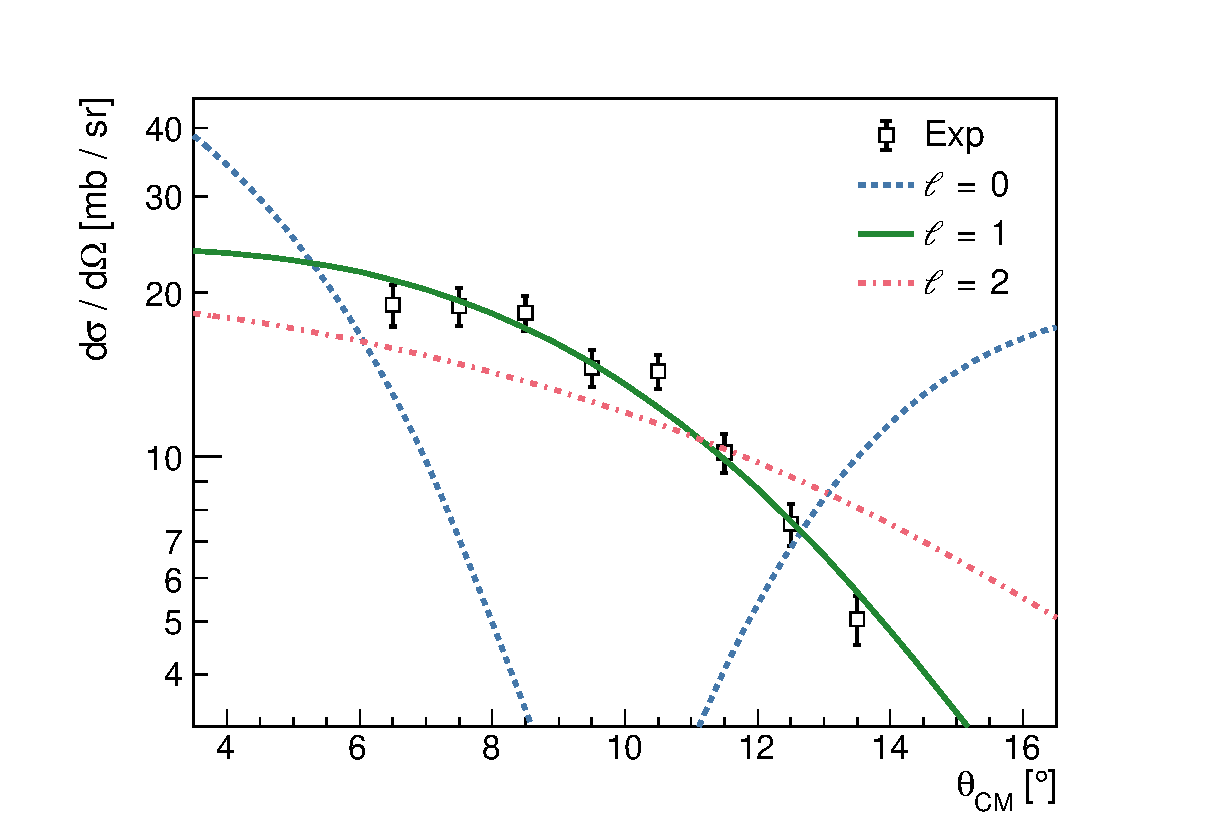
\includegraphics[width=\textwidth]{figures/Workshop/10Be_dt_xs.eps}
            \end{minipage}
        \end{figure}
        \medskip
        \begin{columns}[c]
            \column{0.6\linewidth}
            {
                \begin{itemize}
                    \item \textbf{DWBA} with \textsc{Daehnick} (d) and \textsc{Pang} (t) OMPs
                          % \item Only single-particle overlaps.
                          % \item Finite range calculation.
                    \item \textbf{Best fit} is $\ell = 1$ with $j = 3/2$
                \end{itemize}
            }\hfill
            \column{0.38\linewidth}
            {

                \begin{beamercolorbox}[sep=1ex, center, rounded=true]{boxmyorange}
                    % \textbf{Best fit} is $\ell = 1$\\
                    % with $j = 3/2$.\\
                    $\Rightarrow C^2S = \qty{1.522(44)}{}$
                \end{beamercolorbox}

            }
        \end{columns}

    }
    \only<+>
    {
        \addtocounter{framenumber}{1}
        Another measurement is available in {\small D.L Auton Nucl. Phys. A (1970)}. A reanalysis with \textbf{our model} is executed:

        \begin{figure}
            \centering
            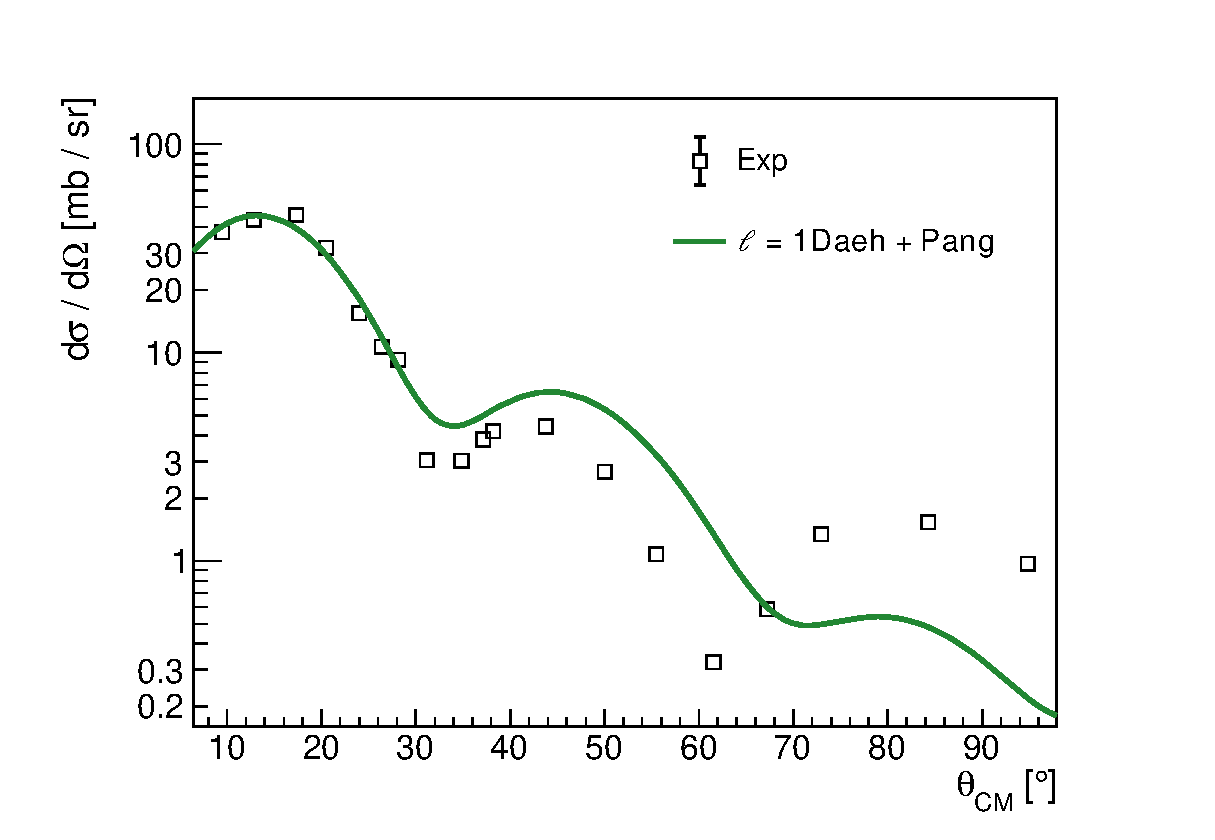
\includegraphics[width=0.5\linewidth]{figures/Workshop/auton.eps}
        \end{figure}
        \medskip
        \begin{columns}[c]
            \column{0.48\linewidth}
            {
                \begin{itemize}
                    \item No errors could be extracted from paper
                    \item Poor quality at large $\theta_{CM}$
                    \item $C^2S = \num{1.951(54)}$
                \end{itemize}

            }
            \hfill
            \column{0.48\linewidth}
            {
                \begin{beamercolorbox}[sep=1ex, center, rounded=true]{boxmyorange}
                    Agreement with our results
                \end{beamercolorbox}
            }
        \end{columns}
    }
\end{frame}

\begin{frame}{Proton removal: $\iso{10}{Be}(\textrm{d}, \iso{3}{He})\iso{9}{Li}$}
    %Three states were observed, although fits are complicated due to low statistics and large $\sigma_{res} \sim \qty{0.75}{\MeV}$. 
    \textbf{E748} can be compared with a recent experiment carried out at the Acculinna facility. For the $E_{x}$:

    \begin{columns}[t]
        \column{0.48\linewidth}
        {
            \begin{figure}
                \captionsetup{belowskip=-8pt}
                \centering
                \caption{Our experiment @ \qty{30}{} AMeV}
                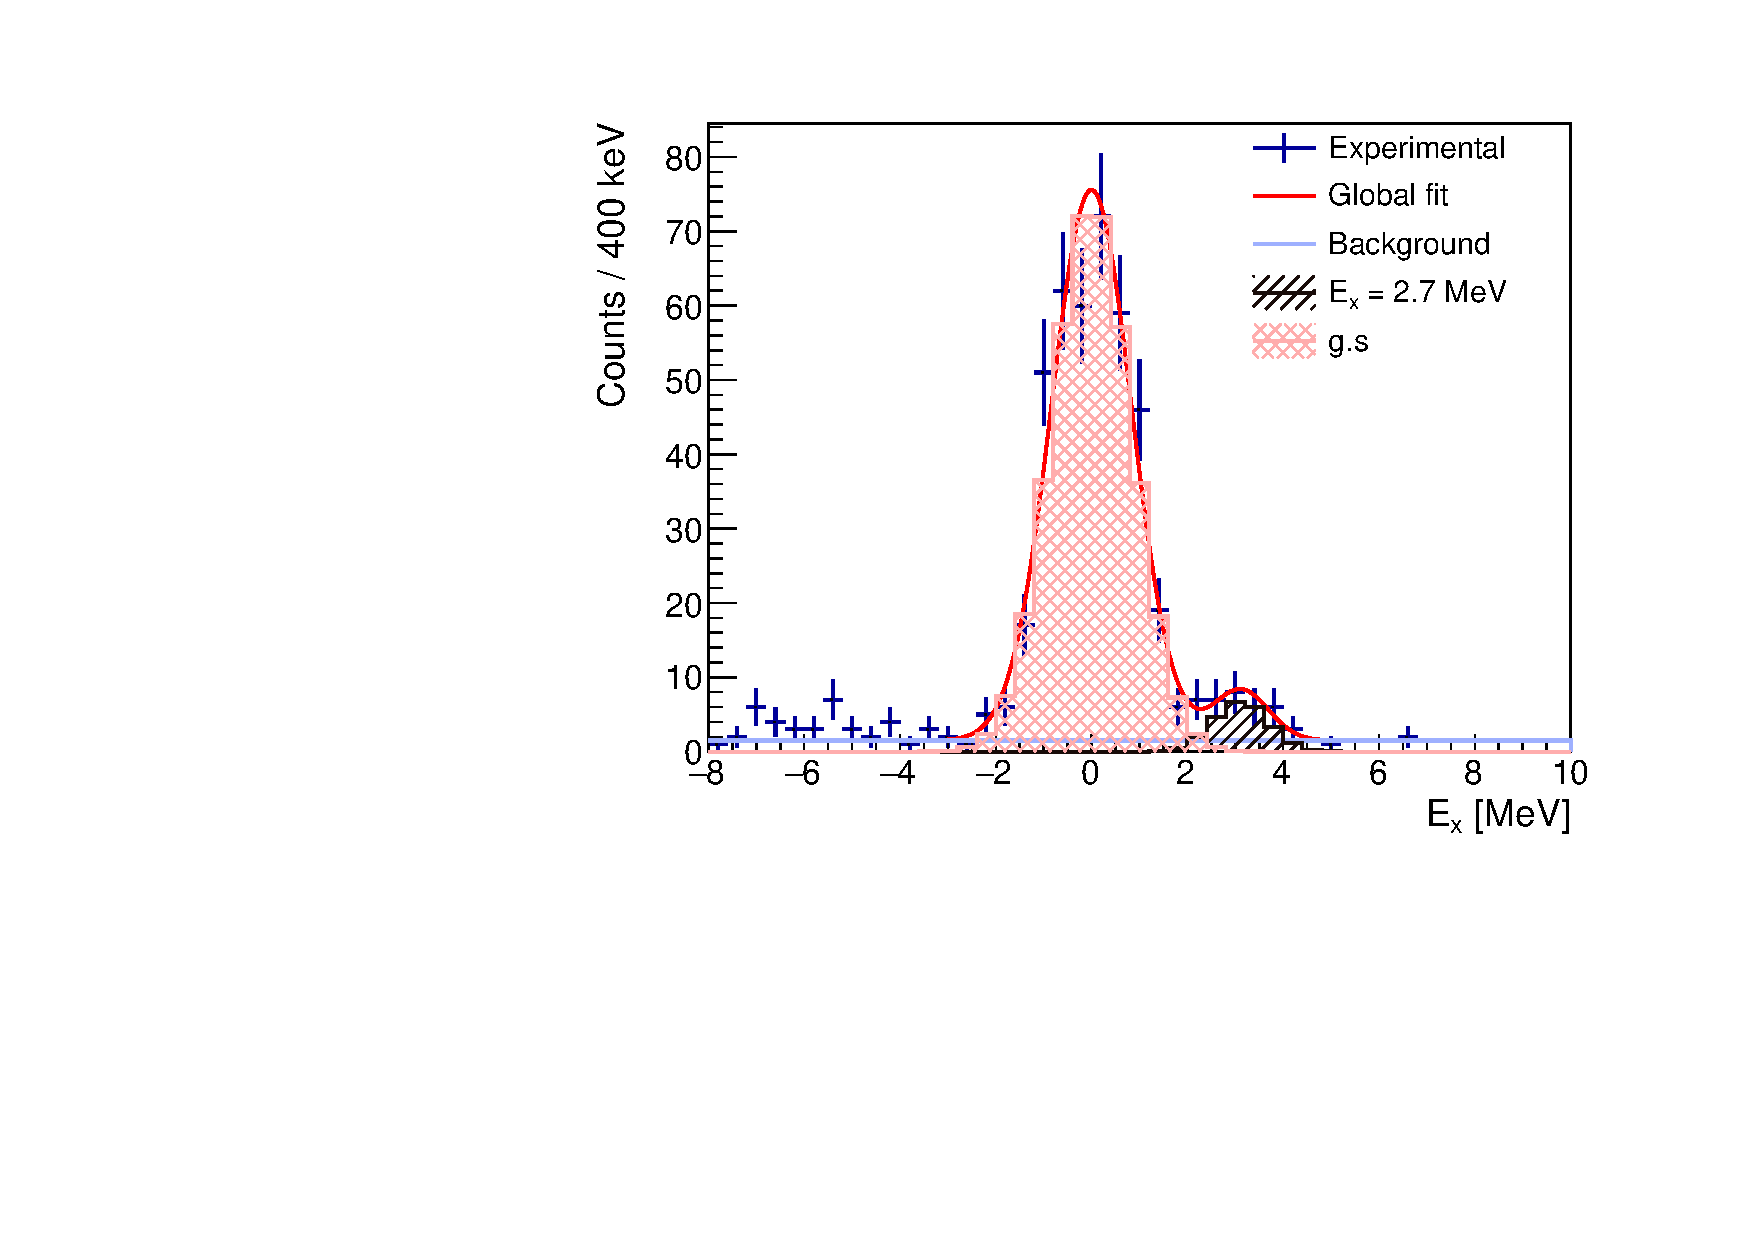
\includegraphics[width=\linewidth, cfbox=myorange 1pt 0pt 0pt]{figures/Workshop/10Be_d3He_ex.pdf}
            \end{figure}
        }
        \hfill
        \column{0.48\linewidth}
        {
            \begin{figure}
                \centering
                \captionsetup{belowskip=2pt}
                \caption{E. Y. Nikolskii et al. @ 42 AMeV}
                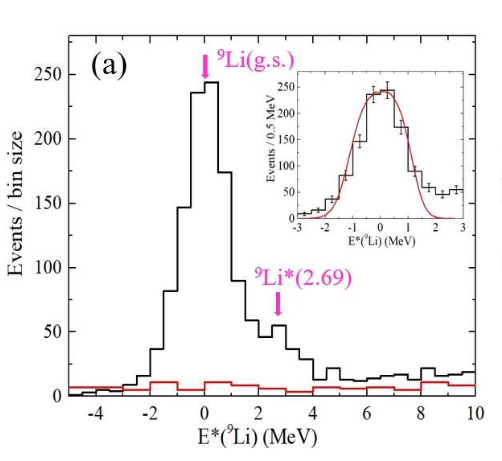
\includegraphics[height=0.41\textheight, cfbox=Mulberry 1pt 1pt]{figures/acculina_new.png}
                \caption{Recently published: NIMPR B 541 (2023)}
            \end{figure}
        }
    \end{columns}

    % \begin{beamercolorbox}[sep=1ex,center, rounded=true, wd=0.48\linewidth]{boxmyorange}
    %     A \textbf{second} excited state is observed!\\
    %     No longer true (CsI disabled)
    % \end{beamercolorbox}

\end{frame}

\begin{frame}{Proton removal: $\iso{10}{Be}(\textrm{d}, \iso{3}{He})\iso{9}{Li}$}
    \only<1,2>{
        Angular distributions for the \textbf{ground state} are extracted:
        \vspace{-\medskipamount}
        \begin{columns}[t]
            \column{0.48\linewidth}
            {
                \begin{figure}
                    \captionsetup{belowskip=-8pt}
                    % \centering
                    % 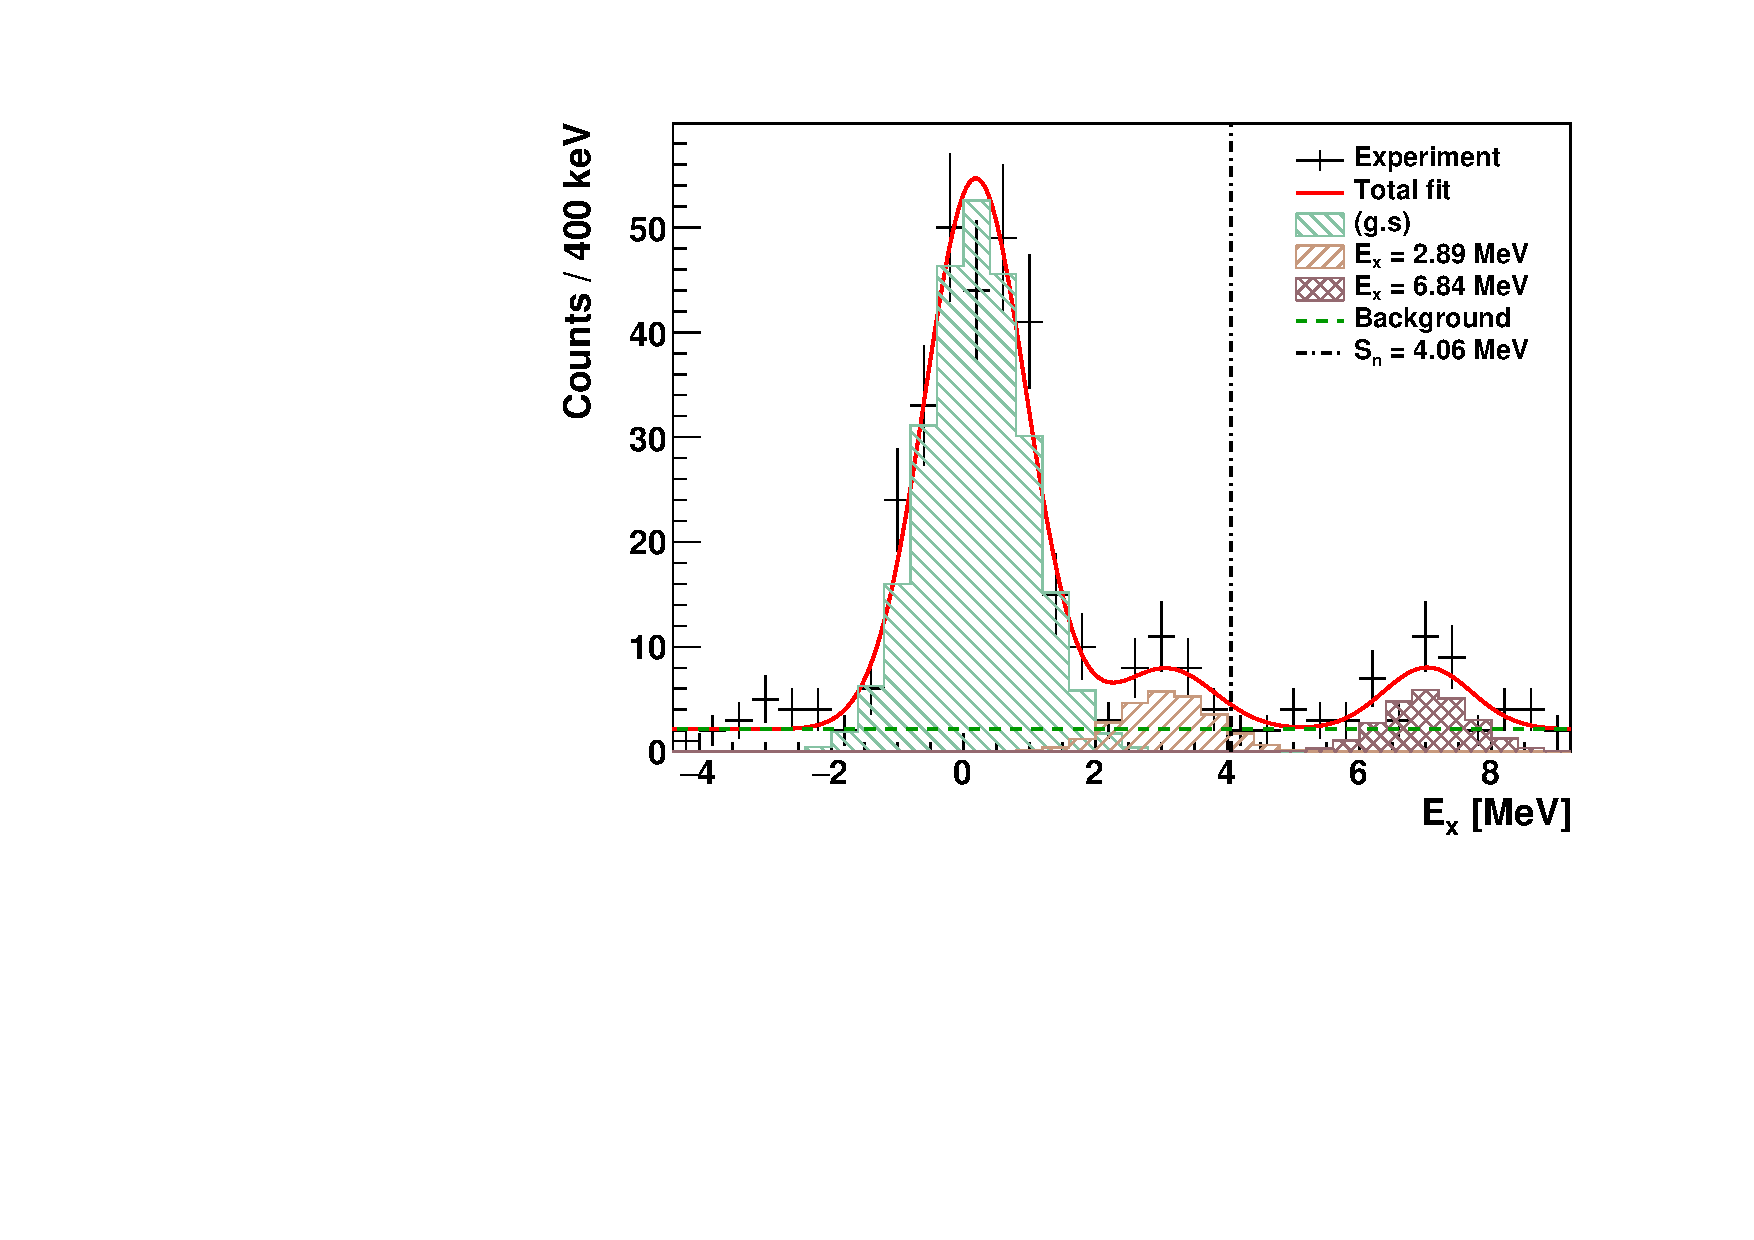
\includegraphics[width=\linewidth]{figures/ex.pdf}
                    \caption{Our experiment, $\theta_{\textrm{CM}} \in \left[6, 14\right]\unit{\degree}$}
                    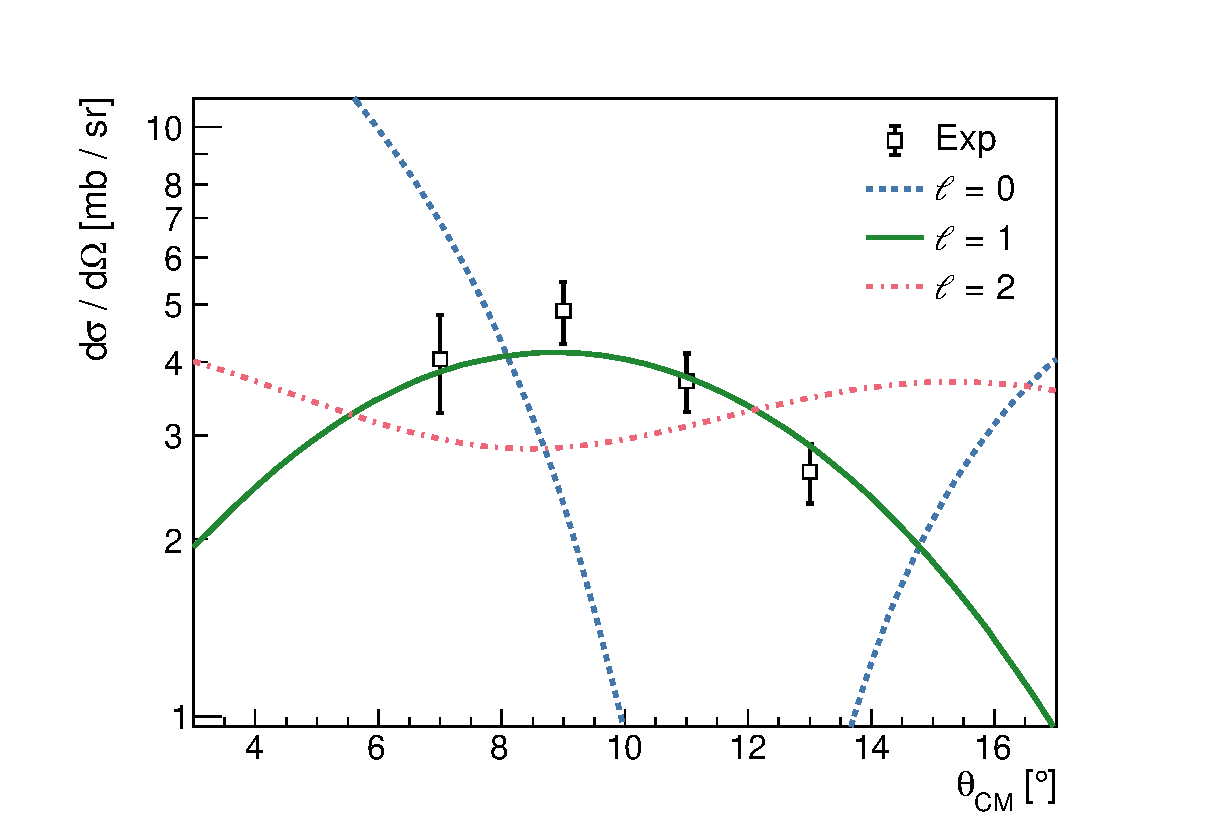
\includegraphics[width=\linewidth, cfbox=myorange 1pt 0pt 0pt]{figures/Workshop/10Be_d3He_xs.eps}
                \end{figure}

                \medskip
                \hfill
                \begin{beamercolorbox}[sep=1ex,center, rounded=true, wd=0.95\linewidth]{boxmyorange}
                    Again $\ell = 1 \implies 3/2^{-}$. \\
                    $C^2S = \qty{1.80(11)}{}$
                \end{beamercolorbox}
                \hfill
            }
            \hfill
            \column{0.48\linewidth}
            {
                \only<1>
                {
                    \begin{figure}
                        \centering
                        \captionsetup{belowskip=3.5pt}
                        \caption{Acculinna one, $\theta_{\textrm{CM}} \in \left[3, 13\right]\unit{\degree}$}
                        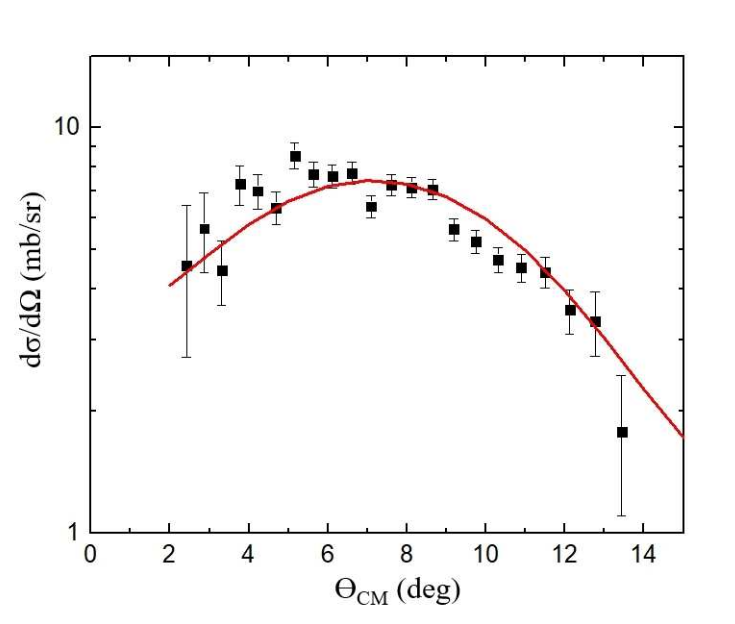
\includegraphics[width=0.8\linewidth, cfbox=Mulberry 1pt 0pt 0pt]{figures/acculina_xs.png}%
                    \end{figure}

                    \medskip
                    \hfill
                    \begin{beamercolorbox}[sep=1ex,center, rounded=true, wd=0.95\linewidth]{boxmyviolet}
                        Original publication:\\
                        $C^2S = \qty{1.74}{}$
                    \end{beamercolorbox}
                    \hfill
                }
                \only<2>
                {
                    \begin{figure}
                        \centering
                        \captionsetup{belowskip=-8pt}
                        \caption{Reanalyis of Acculinna's data}
                        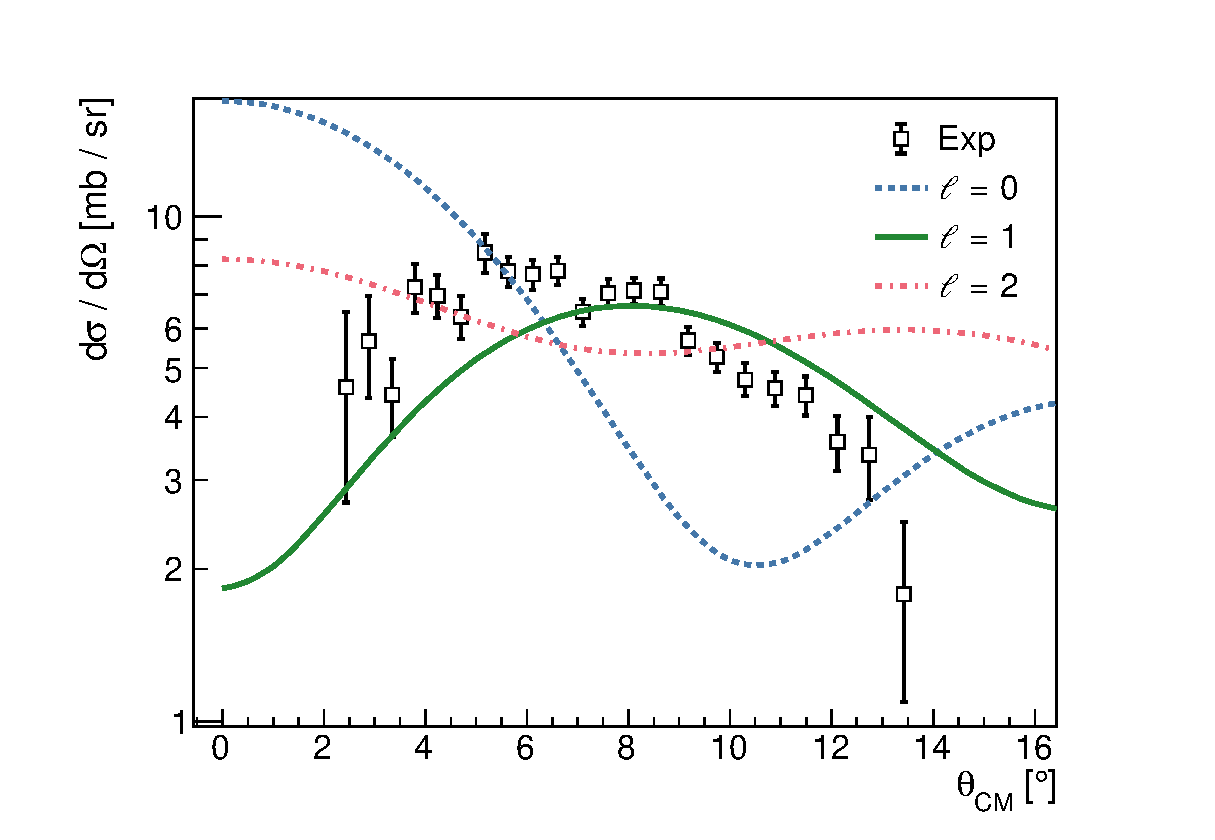
\includegraphics[width=\linewidth, cfbox=Mulberry 1pt 0pt 0pt]{figures/Workshop/acculina.eps}%
                        %\caption{Recently published: NIMPR B 541 (2023)}
                    \end{figure}

                    \medskip
                    \hfill
                    \begin{beamercolorbox}[sep=1ex,center, rounded=true, wd=0.95\linewidth]{boxmyviolet}
                        $\ell = 1 \implies C^2S = \qty{2.679(45)}{}$\\
                        Investigate \textbf{input parameters} in the models!
                    \end{beamercolorbox}
                    \hfill
                }
            }
        \end{columns}
    }
    \only<3>{
        A first excited state is also accesible.
        \begin{columns}[t]
            \column{0.48\linewidth}
            {
                \begin{figure}
                    \centering
                    \begin{tikzpicture}
                        \node[anchor=south west,inner sep=0] (image) at (0,0) {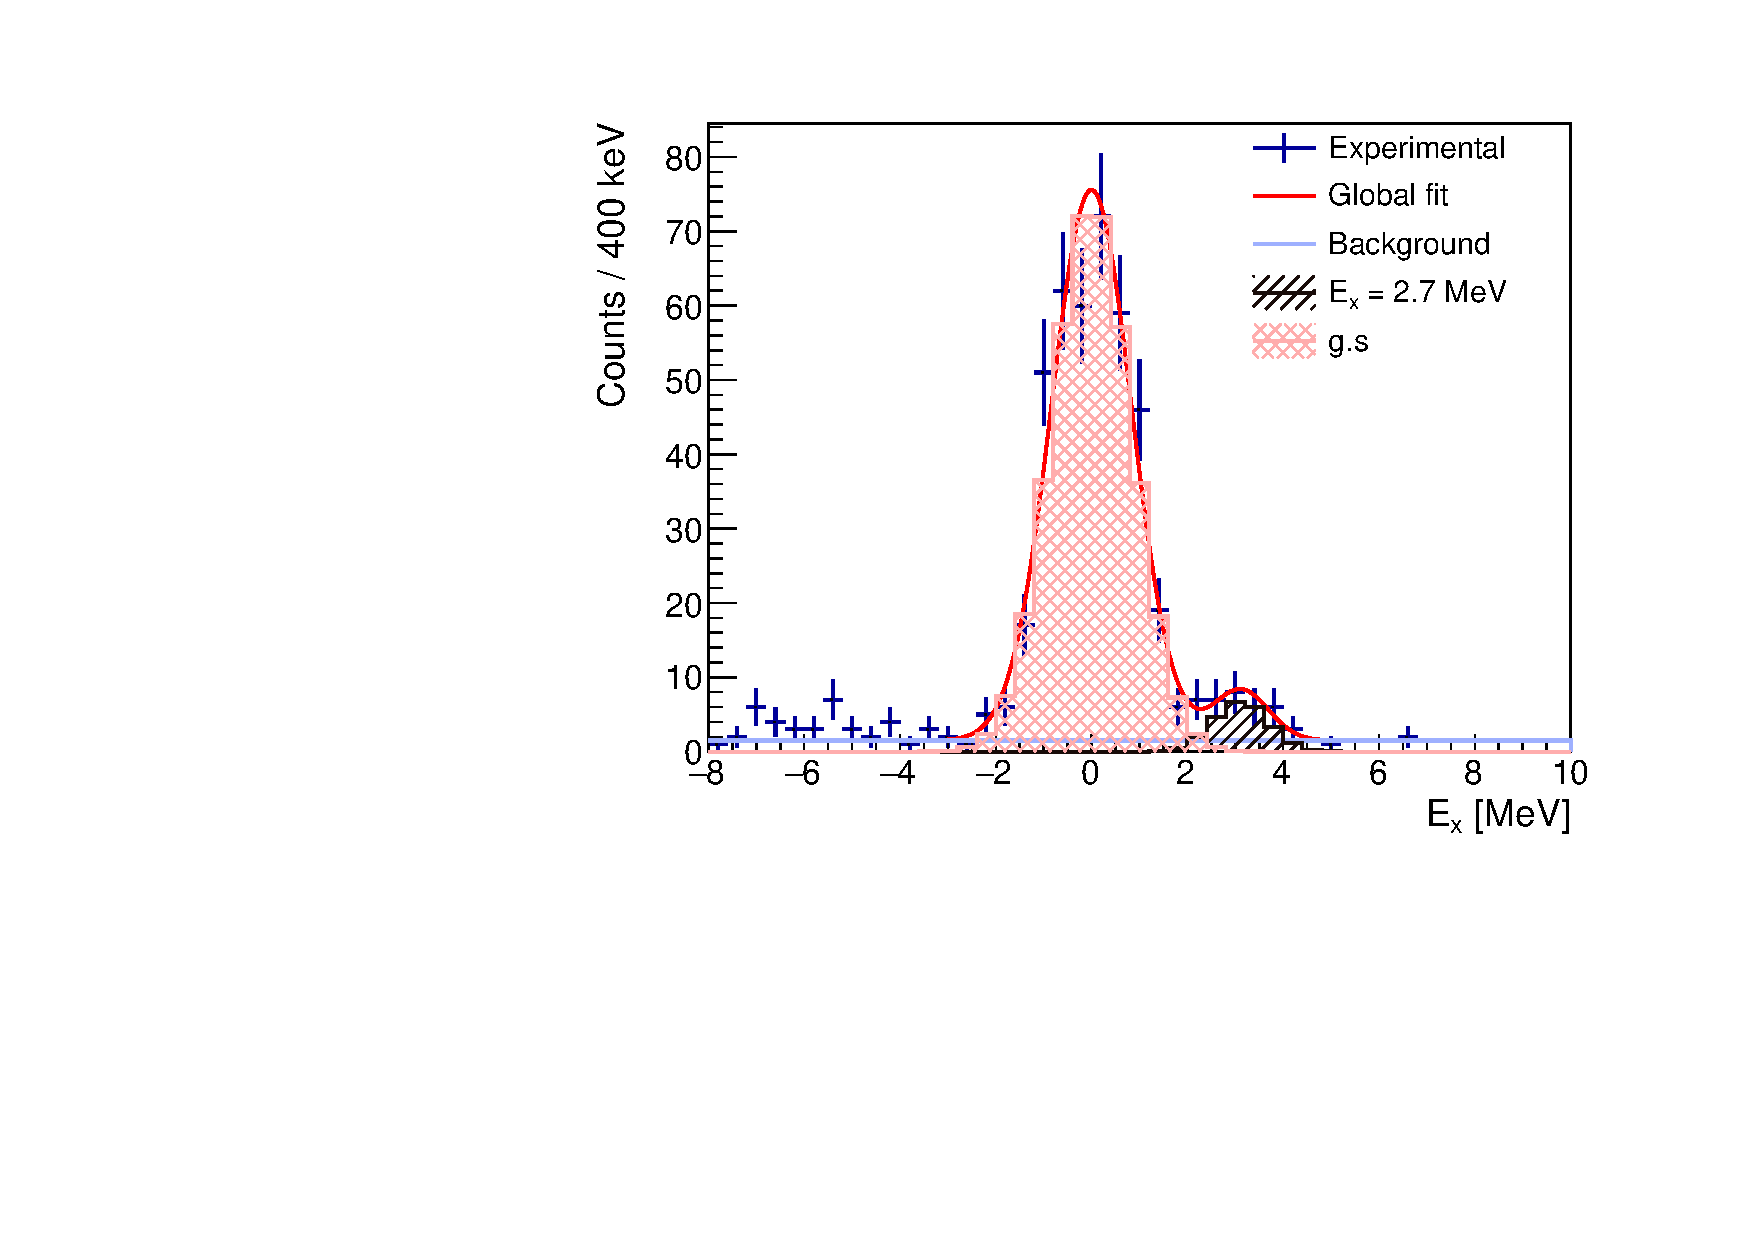
\includegraphics[width=\textwidth]{figures/Workshop/10Be_d3He_ex.pdf}};
                        \begin{scope}[x={(image.south east)},y={(image.north west)}]
                            % \draw[step=0.05,gray,very thin] (0,0) grid (1, 1);
                            \draw[->, very thick, VioletRed] (0.60,0.45) -- (0.60,0.25);
                        \end{scope}
                    \end{tikzpicture}
                \end{figure}
            }
            \hfill
            \column{0.48\linewidth}
            {
                \begin{figure}
                    \centering
                    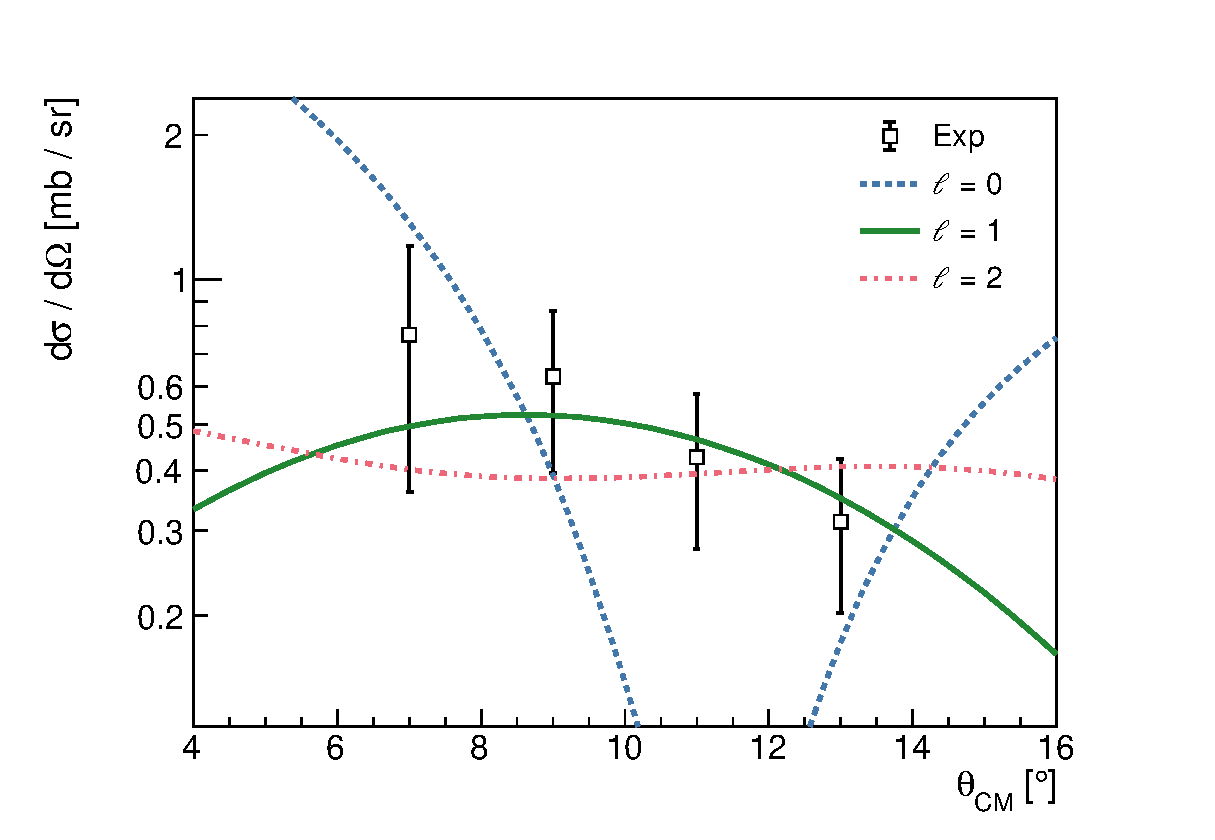
\includegraphics[width=\textwidth]{figures/Workshop/10Be_d3He_xs_1.eps}
                \end{figure}
            }
        \end{columns}

        \begin{itemize}
            \item \textbf{Best fit} is $\ell = 1$
            \item Assuming $j = 1/2$
            \item Spectroscopic factor: \num{0.185(36)}
        \end{itemize}
    }
\end{frame}

\begin{frame}{Elastic: $\iso{12}{Be}(\textrm{d}, \textrm{d})\iso{12}{Be}$}
    \only<+>{
        Yet another validation method of the normalization.
        \begin{figure}
            \begin{minipage}[t]{0.48\linewidth}
                \centering
                \begin{tikzpicture}
                    \node[anchor=south west,inner sep=0] (image) at (0,0) {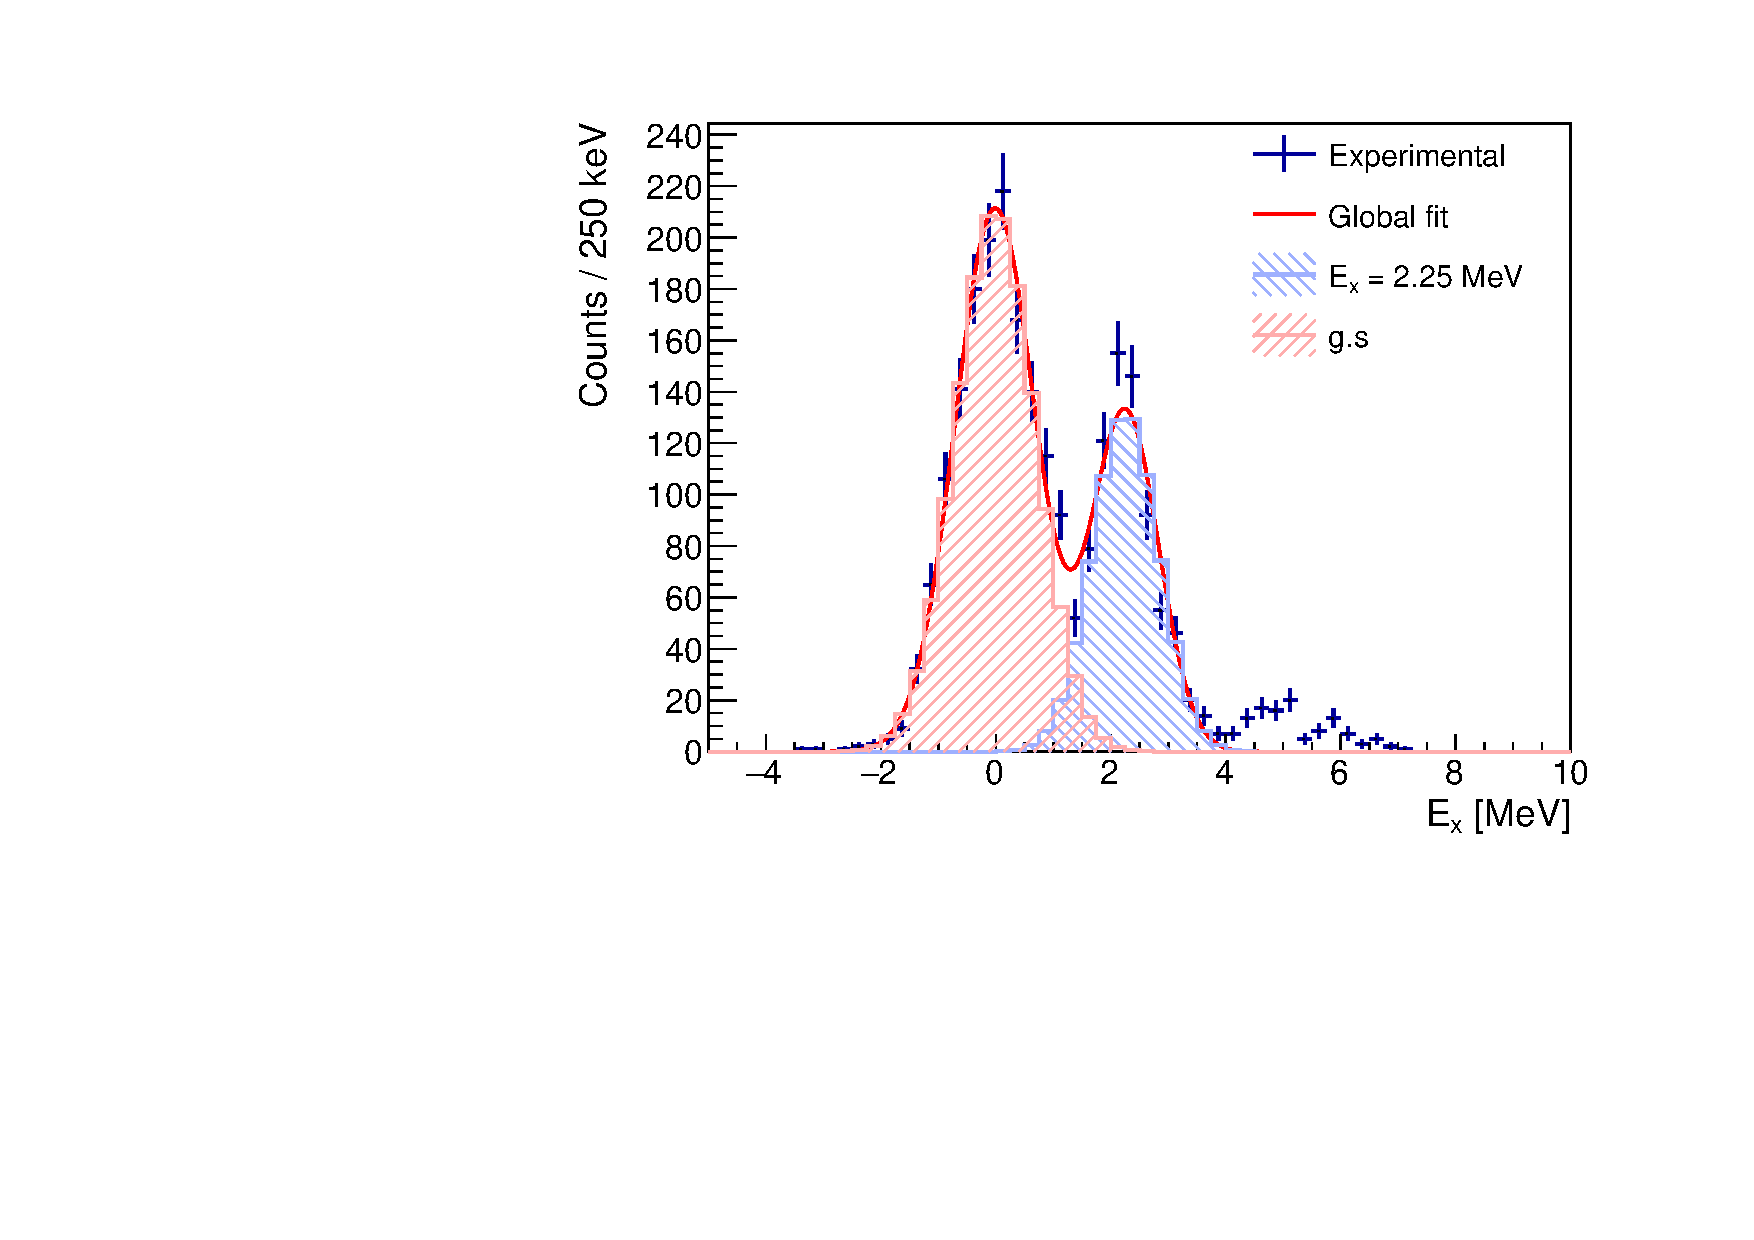
\includegraphics[width=\textwidth]{figures/Workshop/12Be_dd_ex.pdf}};
                    \begin{scope}[x={(image.south east)},y={(image.north west)}]
                        % \draw[step=0.05,gray,very thin] (0,0) grid (1, 1);
                        \draw[->, very thick, VioletRed] (0.39,0.99) -- (0.39,0.86);
                    \end{scope}
                \end{tikzpicture}
            \end{minipage}
            \hfill
            \begin{minipage}[t]{0.48\linewidth}
                \centering
                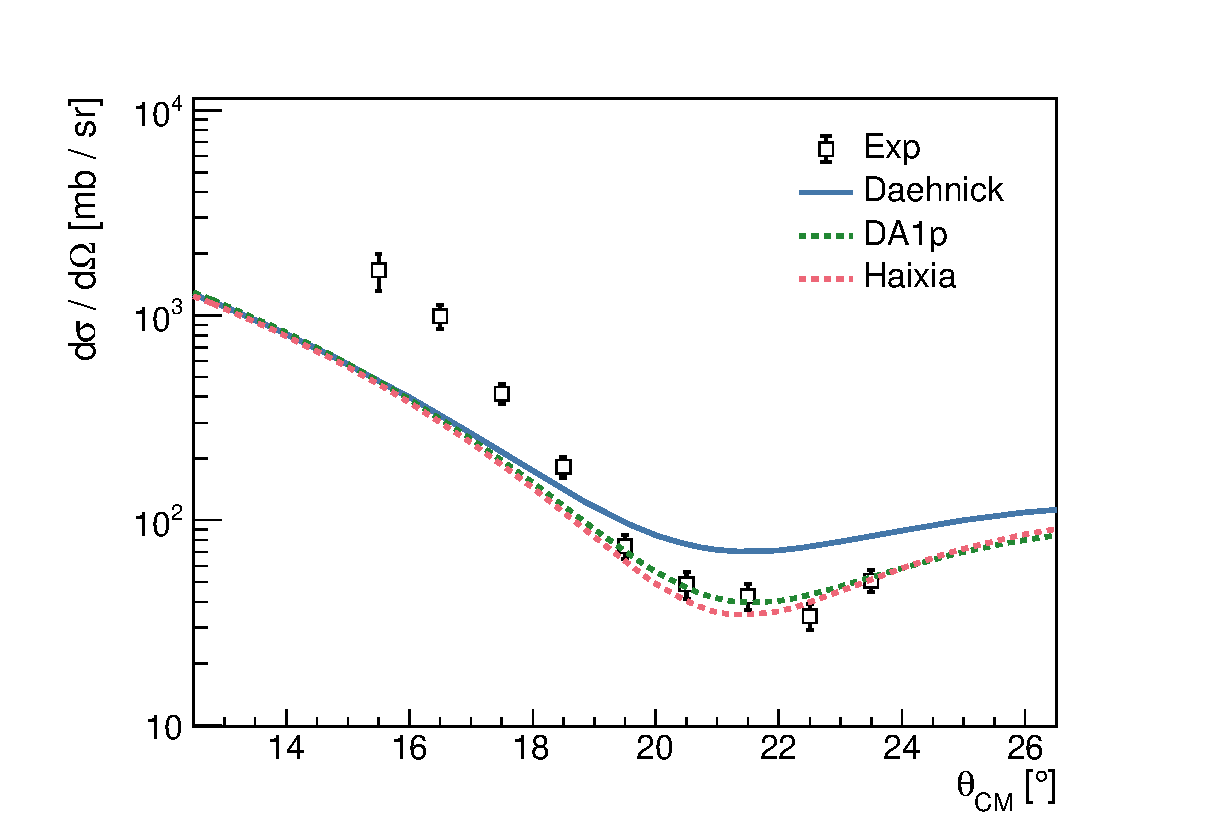
\includegraphics[width=\textwidth]{figures/Workshop/12Be_dd_xs.eps}
            \end{minipage}
        \end{figure}
        \begin{columns}
            \column{0.58\linewidth}
            {
                \begin{itemize}
                    \item Same behaviour as for \iso{10}{Be}
                    \item Normalization fine for this beam also
                \end{itemize}
            }\hfill
            \column{0.38\linewidth}
            {
                \begin{beamercolorbox}[sep=1ex, center, rounded=true]{boxmyorange}
                    Clearly the same \textit{systematic} error
                \end{beamercolorbox}

            }
        \end{columns}
    }
    \only<+>{
        Cross-section for the 1st excited state is also achievable.
        \begin{figure}
            \begin{minipage}[t]{0.48\linewidth}
                \centering
                \begin{tikzpicture}
                    \node[anchor=south west,inner sep=0] (image) at (0,0) {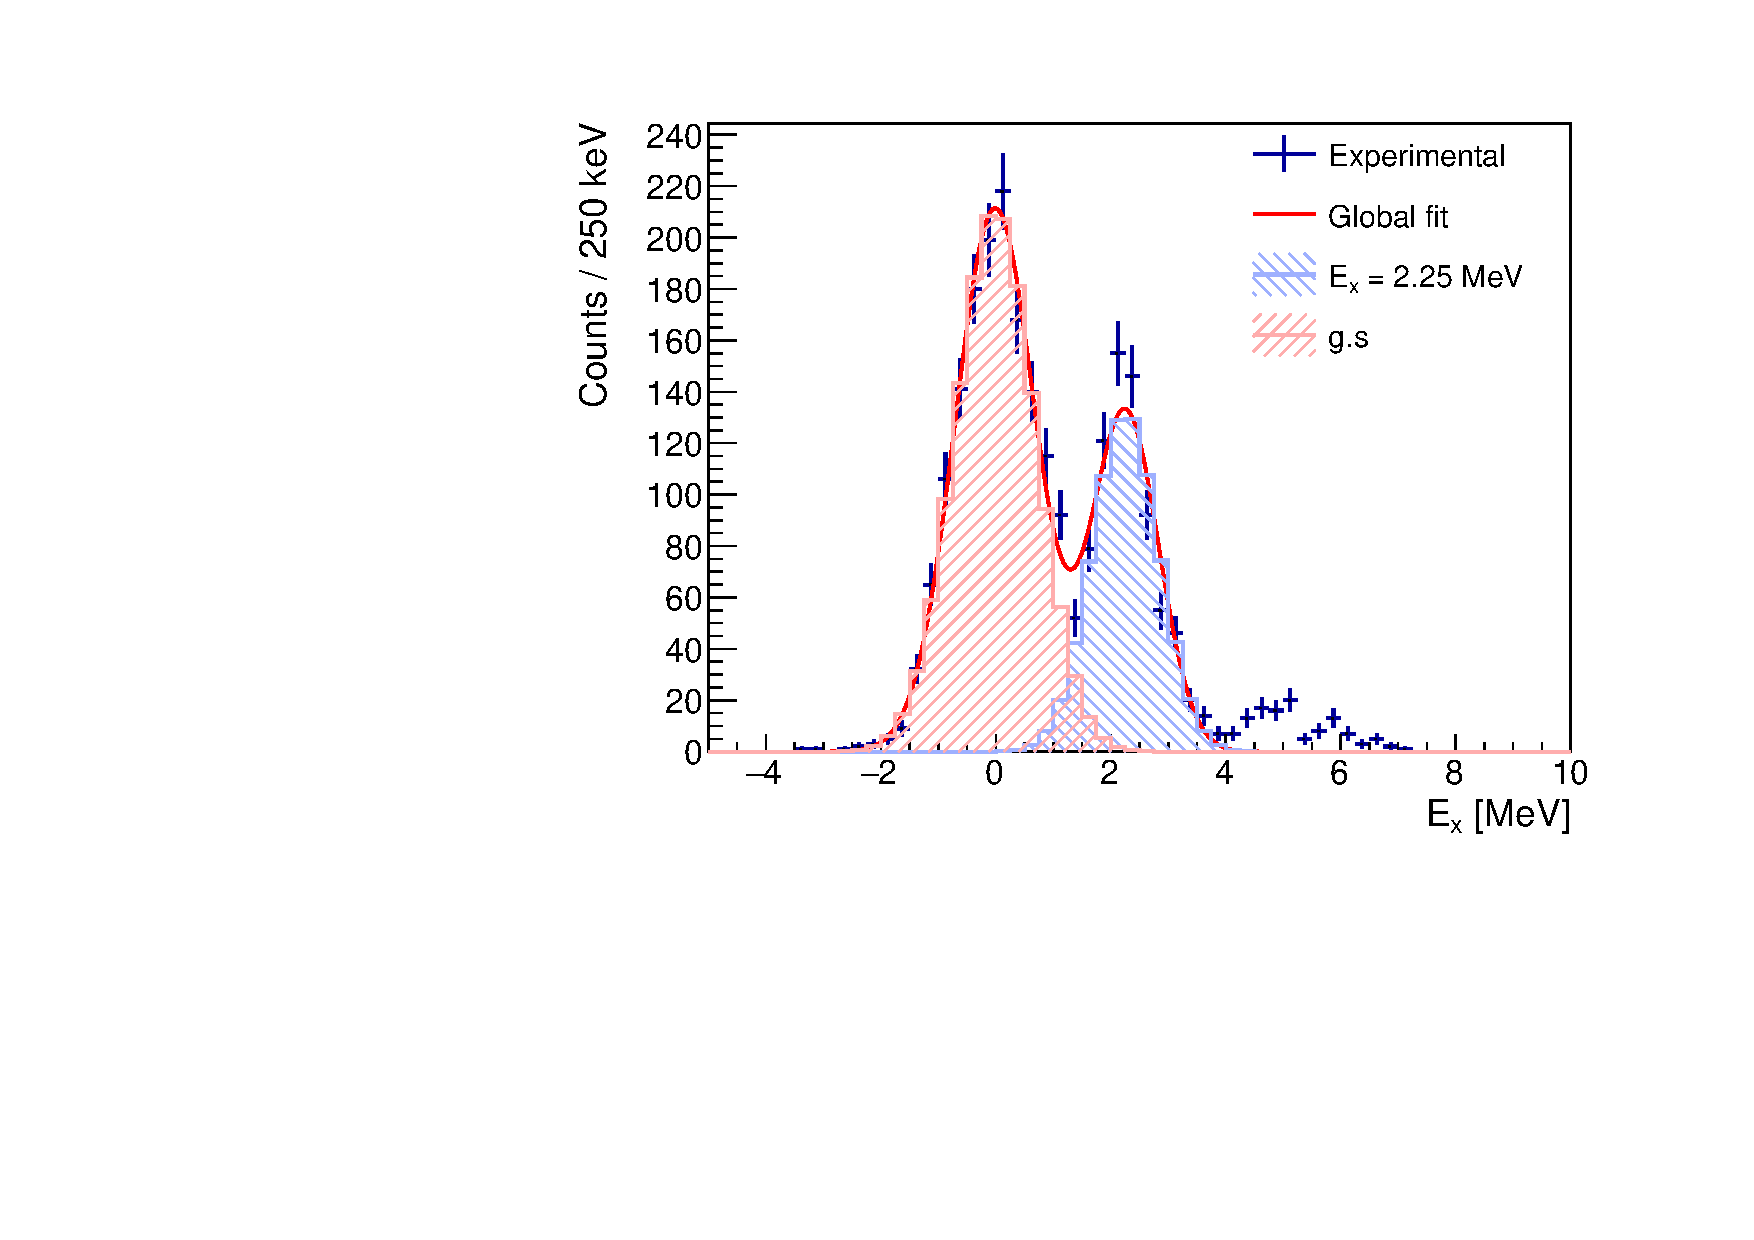
\includegraphics[width=\textwidth]{figures/Workshop/12Be_dd_ex.pdf}};
                    \begin{scope}[x={(image.south east)},y={(image.north west)}]
                        % \draw[step=0.05,gray,very thin] (0,0) grid (1, 1);
                        \draw[->, very thick, VioletRed] (0.50,0.84) -- (0.50,0.65);
                    \end{scope}
                \end{tikzpicture}
            \end{minipage}
            \hfill
            \begin{minipage}[t]{0.48\linewidth}
                \centering
                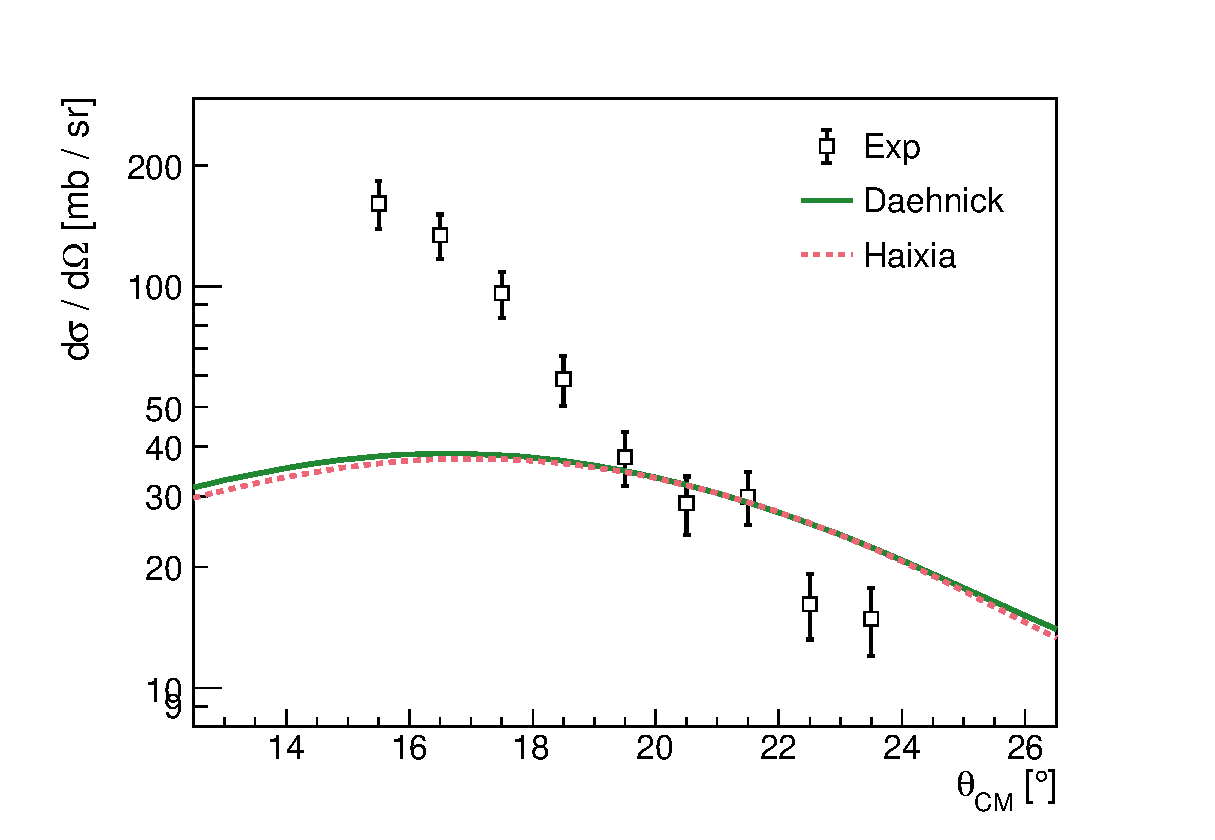
\includegraphics[width=\textwidth]{figures/Workshop/12Be_dd_xs_g1.eps}
            \end{minipage}
        \end{figure}
        \begin{columns}
            \column{0.58\linewidth}
            {
                \begin{itemize}
                    \item Same procedure as before
                \end{itemize}
            }\hfill
            \column{0.38\linewidth}
            {

                \begin{beamercolorbox}[sep=1ex, center, rounded=true]{boxmyorange}
                    To be further investigated. \\
                    $\Rightarrow C^2S = \qty{0.519(30)}{}$ with Daehnick
                \end{beamercolorbox}

            }
        \end{columns}
    }
\end{frame}

\begin{frame}{Challenging channels: $\iso{12}{Be}(\textrm{d}, \textrm{t})\iso{11}{Be}$}
    \begin{figure}
        \centering
        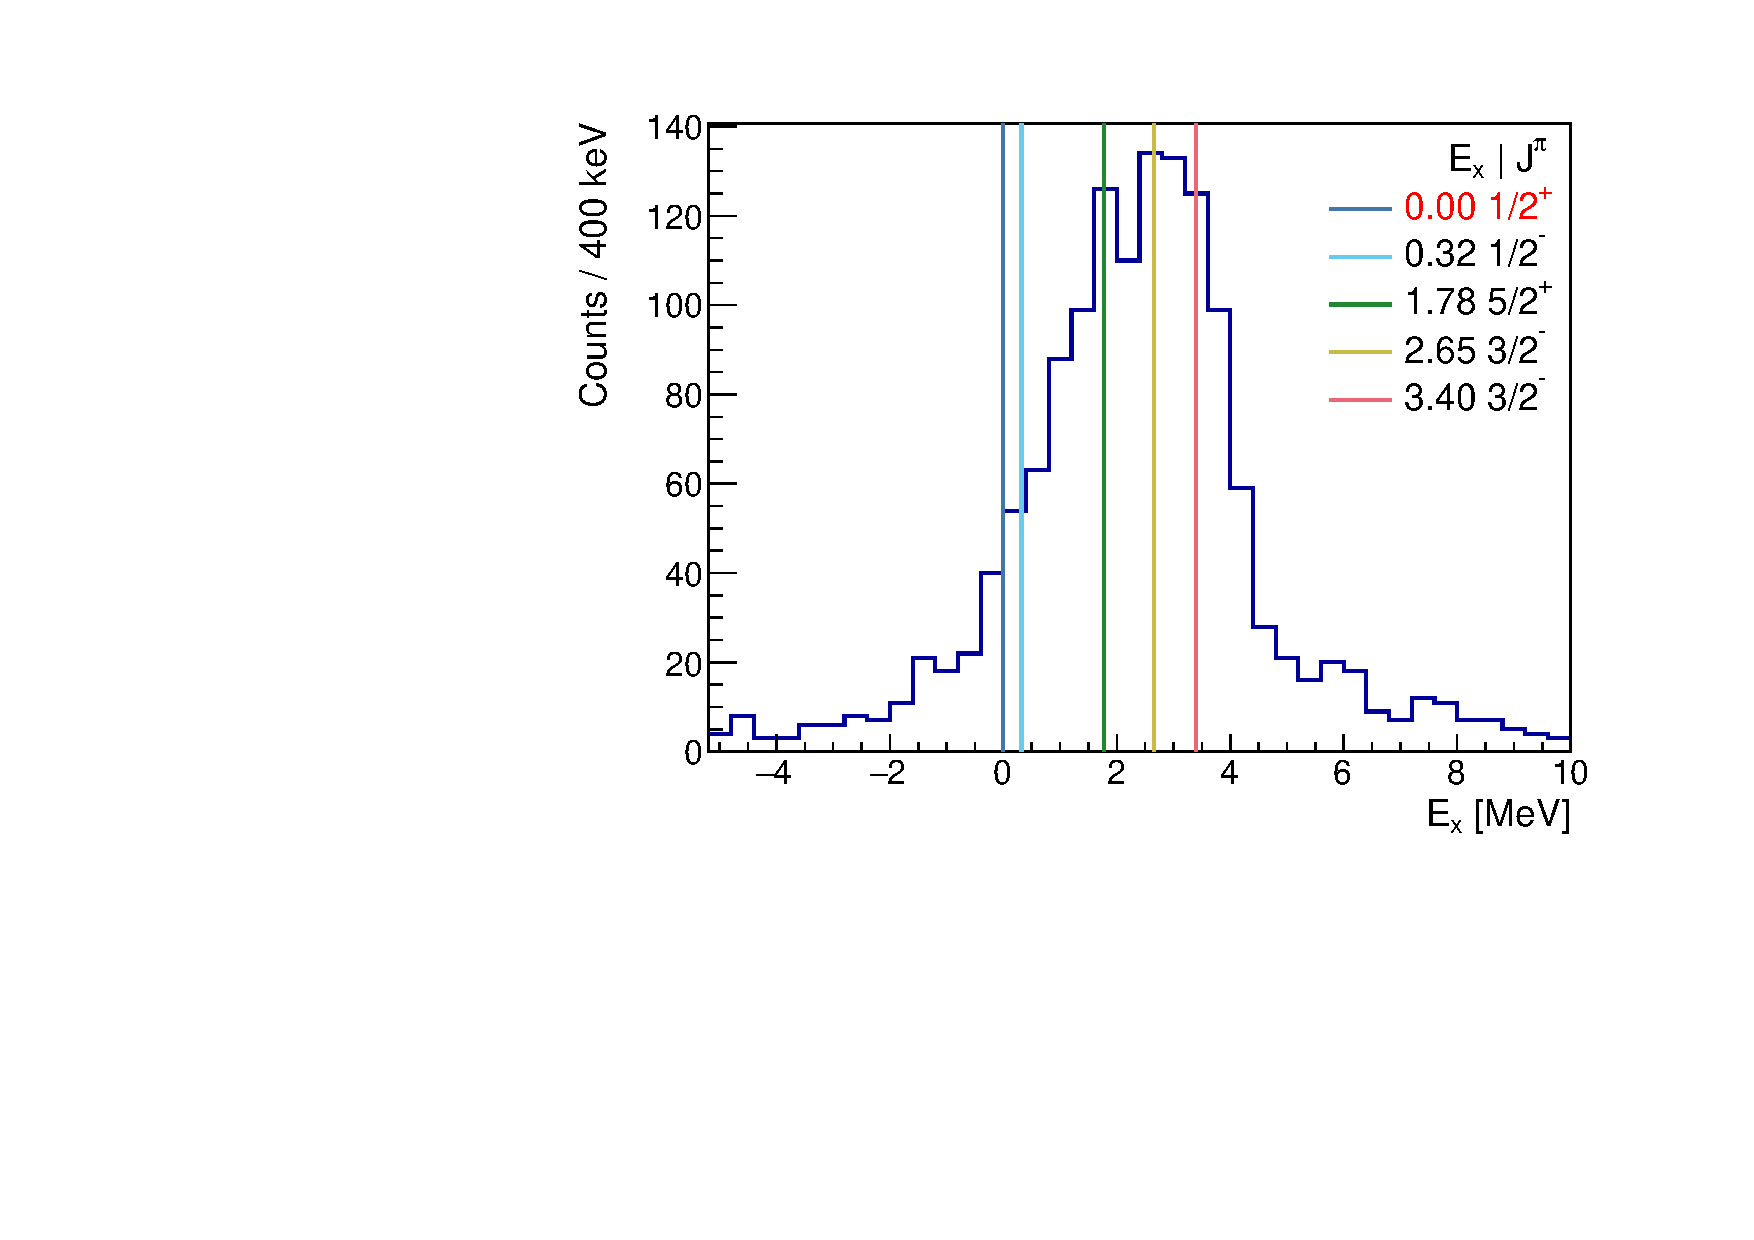
\includegraphics[width=0.6\linewidth]{figures/Workshop/12Be_dt_ex.pdf}
    \end{figure}
    \medskip
    \begin{itemize}
        \item Strong \textbf{inhibition} of the ground state
        \item Why? Related to parity inversion in \iso{11}{Be}?
    \end{itemize}
\end{frame}

\begin{frame}{Challenging channels: $\iso{12}{Be}(\textrm{d}, \iso{3}{He})\iso{11}{Li}$}
    \begin{figure}
        \begin{minipage}[t]{0.48\linewidth}
            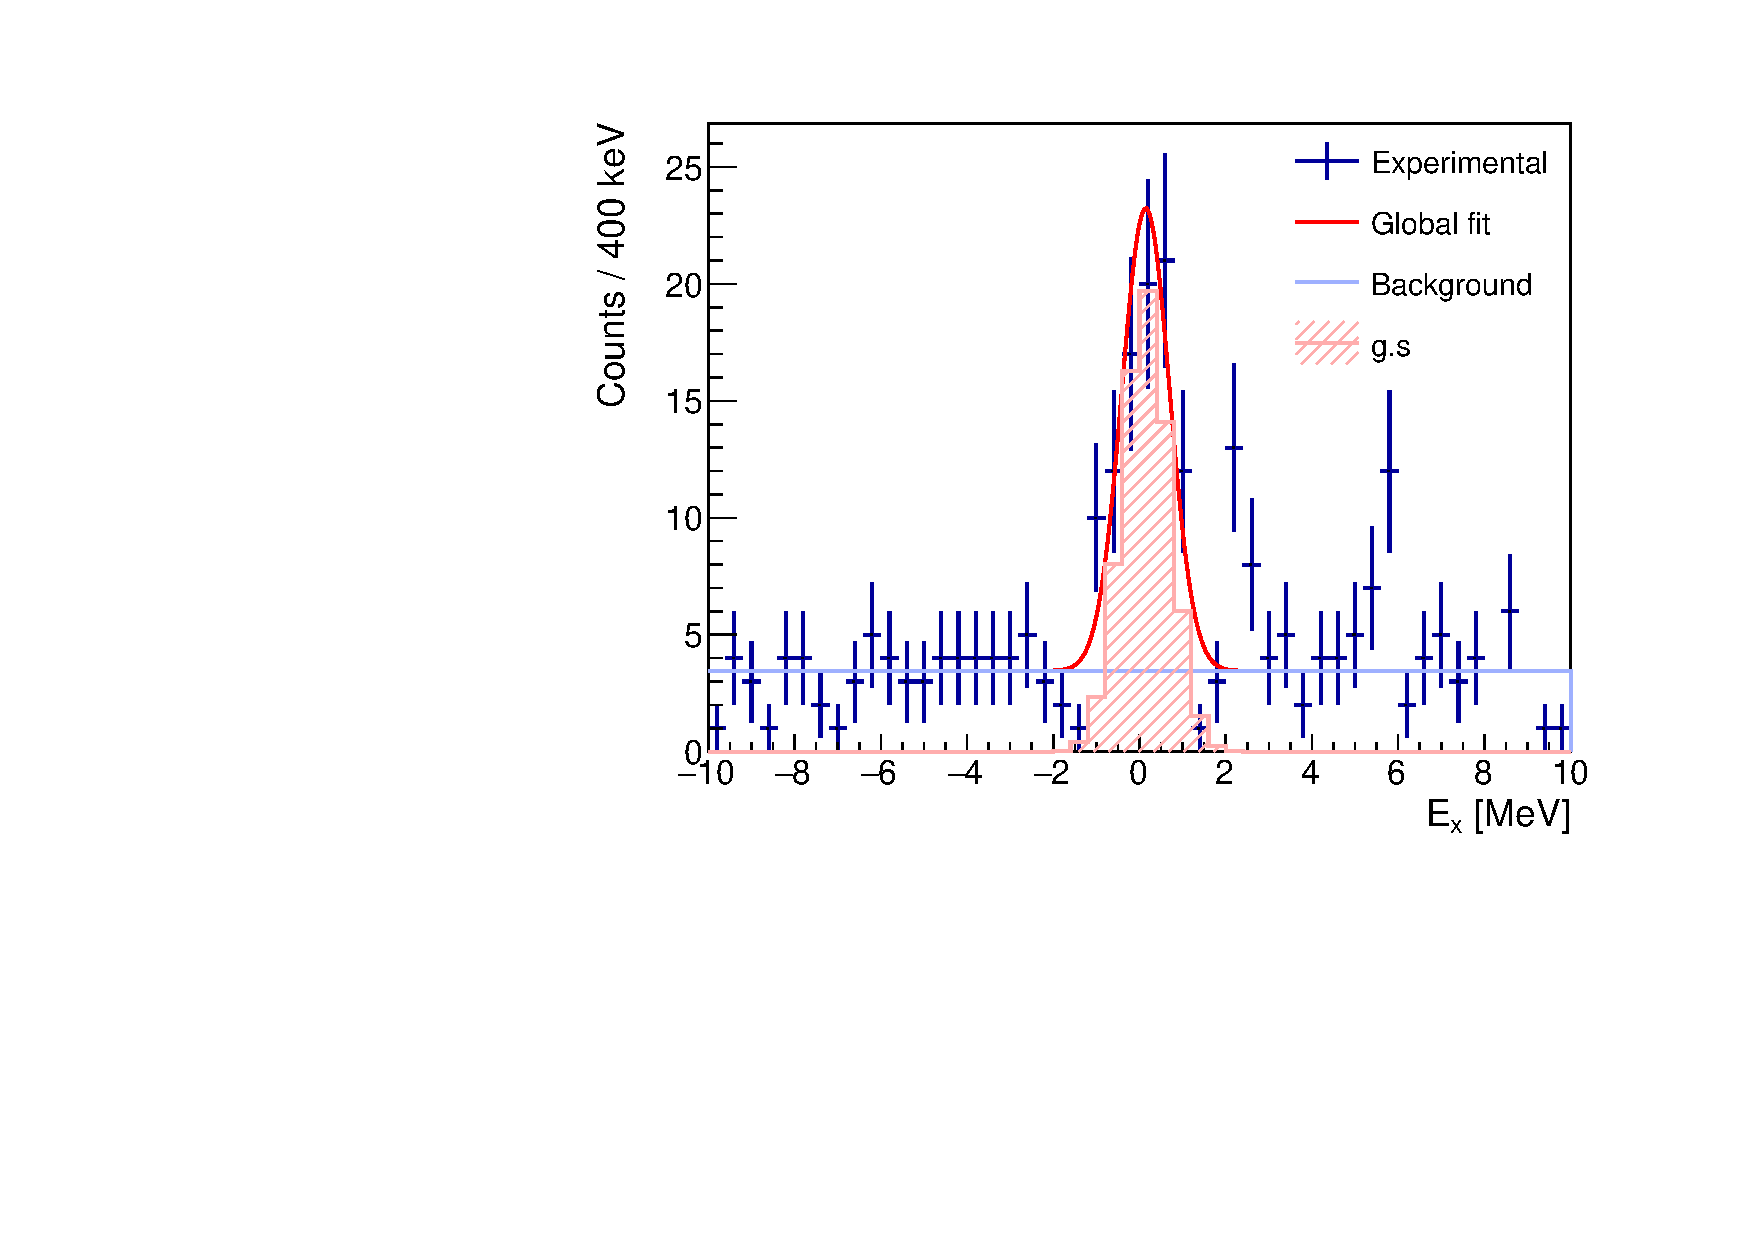
\includegraphics[width=\textwidth]{figures/Workshop/12Be_d3He_ex.pdf}
        \end{minipage}
        \hfill
        \begin{minipage}[t]{0.48\linewidth}
            \centering

            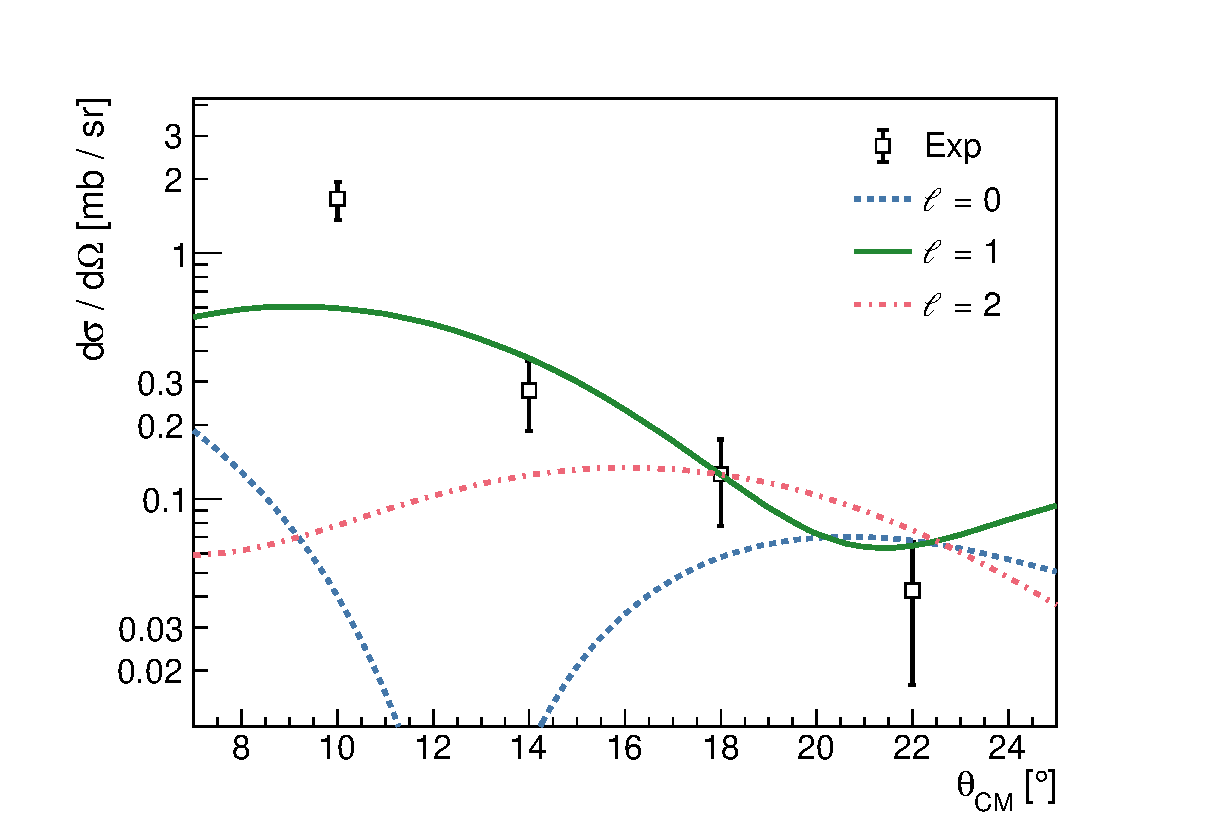
\includegraphics[width=\textwidth]{figures/Workshop/12Be_d3He_xs.eps}
        \end{minipage}
    \end{figure}
    \bigskip
    \begin{columns}[c]
        \column{0.48\linewidth}
        {
            \begin{itemize}
                \item Low cross-section
                \item Subject to \textbf{contamination}: hard to disentangle $A = 3$
            \end{itemize}
        }\hfill
        \column{0.48\linewidth}
        {
            \begin{beamercolorbox}[sep=1ex, center, rounded=true]{boxmyviolet}
                $\Rightarrow C^2S = \qty{0.510(85)}{}$ with Daehnick
            \end{beamercolorbox}
        }
    \end{columns}
\end{frame}

\Section{Outlook}
\begin{frame}[c]{Conclusions and outlook}
    \only<+>{
        We investigated several proton and neutron pick-up reactions on \iso{10,12}{Be}:
        \bigskip
        \begin{table}
            \centering
            \begin{tabular}{@{}ccccc@{}}
                \toprule
                                      & Channel  & Status           & Pending                        & \\ \midrule
                \multirow{3}{*}{10Be} & (d,d)    & Normalization OK & Requires study                 & \\
                                      & (d,t)    & Completed        & $C^2S$ matches other measures. & \\
                                      & (d, 3He) & Completed        & Two new $C^2S$                 & \\ \midrule
                \multirow{3}{*}{12Be} & (d,d)    & Normalization OK & Same as \iso{10}{Be}           & \\
                                      & (d,t)    & Puzzled          & ?                              & \\
                                      & (d,3He)  & Needs clean      & New $C^2S$                     & \\ \bottomrule
            \end{tabular}
            % \caption{}
            % \label{tab:my-table}
        \end{table}
    }
    \only<+>{
        \begin{center}
            \textbf{Future prospects}
            
            ~
            \bigskip
            \begin{beamercolorbox}[sep=1.25ex,center, rounded=true, wd=0.7\linewidth]{boxgreenish}
                Solve discrepancies in \textbf{elastic} channels
            \end{beamercolorbox}
            \bigskip
            \begin{beamercolorbox}[sep=1.25ex,center, rounded=true, wd=0.7\linewidth]{boxpinky}
                Reduce contamination in \iso{3}{He} PID
            \end{beamercolorbox}
            \bigskip
            \begin{beamercolorbox}[sep=1.25ex,center, rounded=true, wd=0.7\linewidth]{boxmyorange}
                Compare with \textbf{shell model} calculations
            \end{beamercolorbox}


            % \begin{columns}[c]
            %     \column{0.3\linewidth}
            %     {
            %         \begin{beamercolorbox}[sep=1.25ex,center, rounded=true, wd=\linewidth]{boxgreenish}
            %             Extract $\frac{\textrm{d}\sigma}{\textrm{d}\Omega}$ for \textbf{excited} states.
            %         \end{beamercolorbox}
            %     }
            %     \hfill
            %     \column{0.3\linewidth}
            %     {
            %         \begin{beamercolorbox}[sep=1.25ex,center, rounded=true, wd=\linewidth]{boxgreenish}
            %             In-detail study of $\iso{12}{Be}(\textrm{d}, \textrm{t})\iso{11}{Be}$.
            %         \end{beamercolorbox}
            %     }
            %     \hfill
            %     \column{0.3\linewidth}
            %     {
            %         \begin{beamercolorbox}[sep=1.25ex,center, rounded=true, wd=\linewidth]{boxgreenish}
            %             Comprehensive analysis of the employed \textbf{reaction model}.
            %         \end{beamercolorbox}
            %     }
            %     \hfill
            % \end{columns}
        \end{center}
    }
\end{frame}

\End
\begin{frame}[plain,standout]
    \centering
    \textbf{Thanks for your attention!}\\
    And special thanks to the \textbf{\itshape\scshape e748} collaboration.
\end{frame}

\begin{frame}[plain, standout]
    \centering
    \textbf{Not part of the talk!}
\end{frame}

\begin{frame}[c]{CsI on or off?}
    So far, studied excited states are \textit{compressed} in the DSSD layer:

    \begin{minipage}[t]{0.48\linewidth}
        \centering
        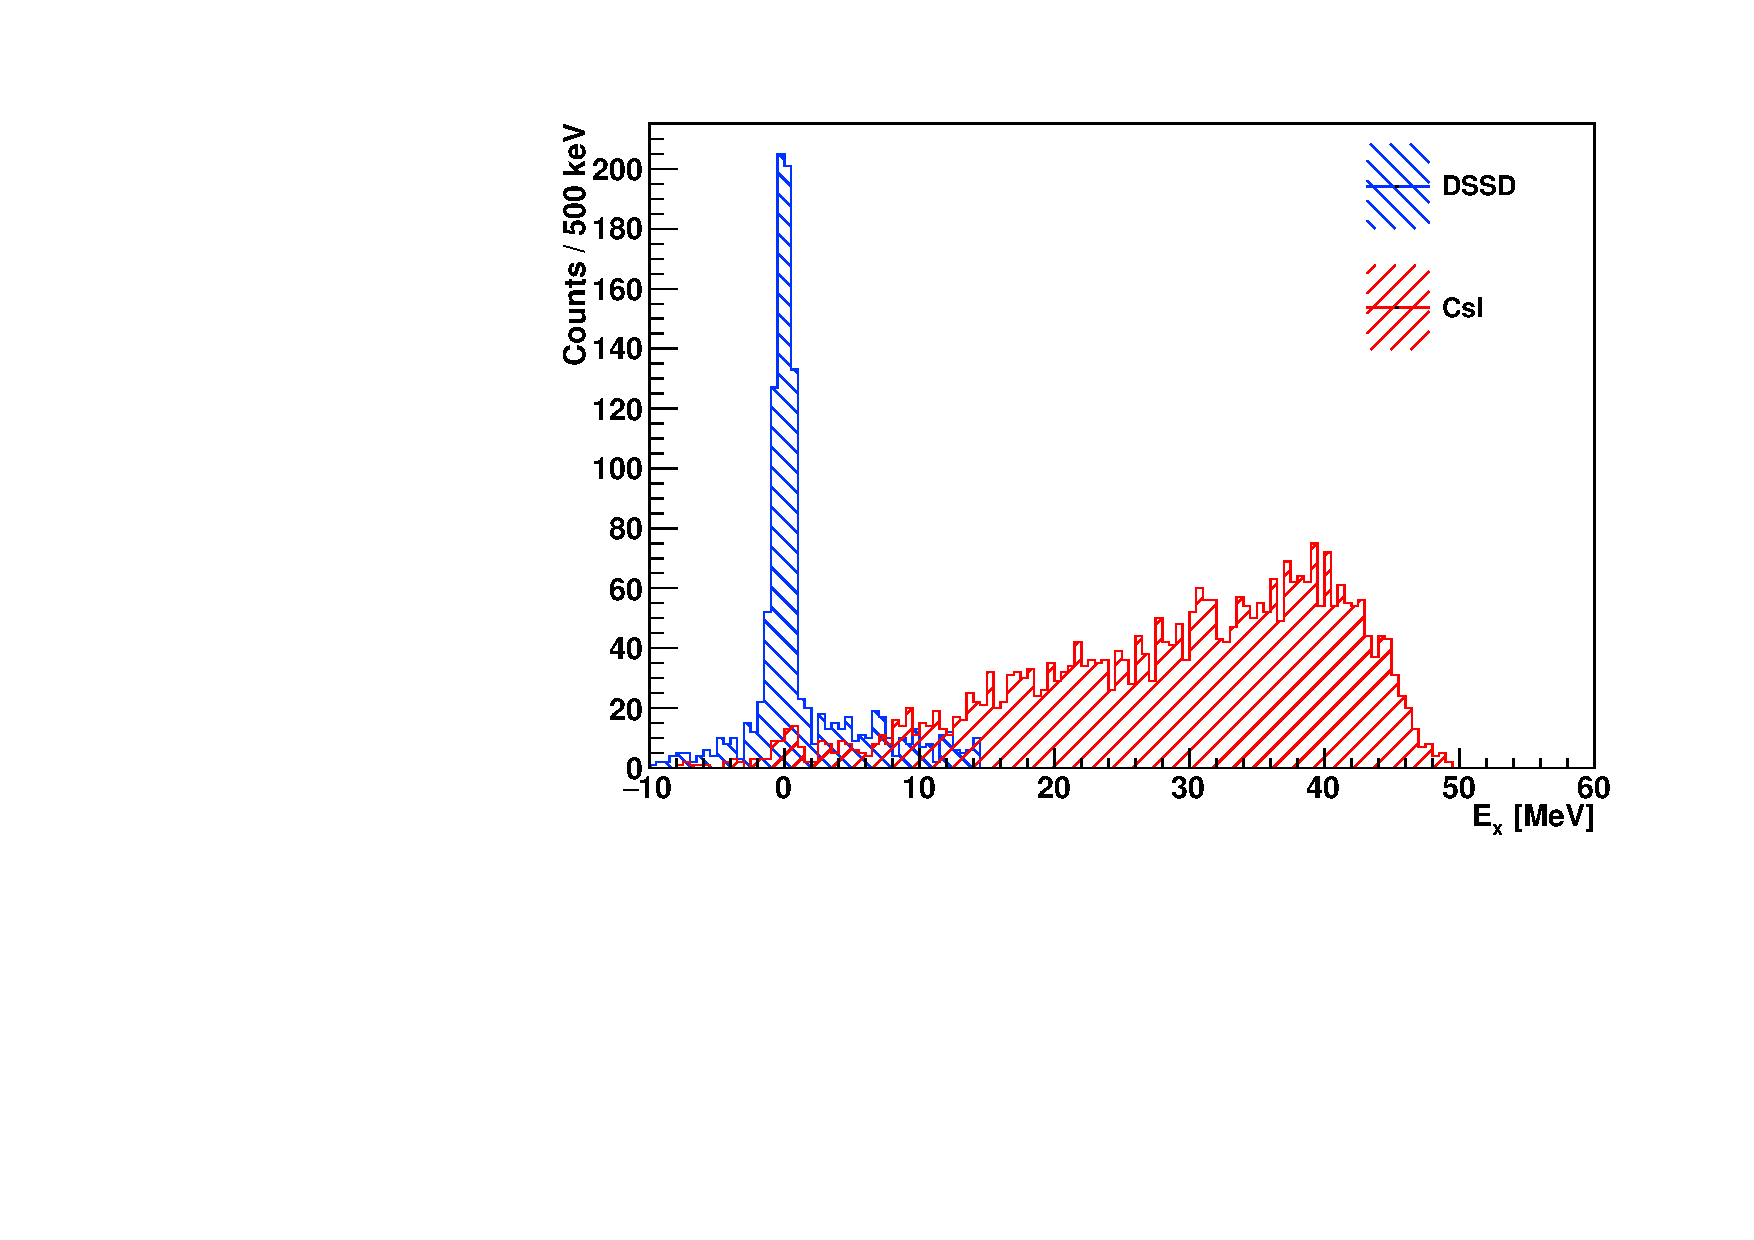
\includegraphics[width=\textwidth]{figures/with_without_csi_9Be.pdf}
        \captionof{figure}{For \iso{10}{Be}(d, t)\iso{9}{Be}}
    \end{minipage}%
    \hfill
    \begin{minipage}[t]{0.48\linewidth}
        \centering
        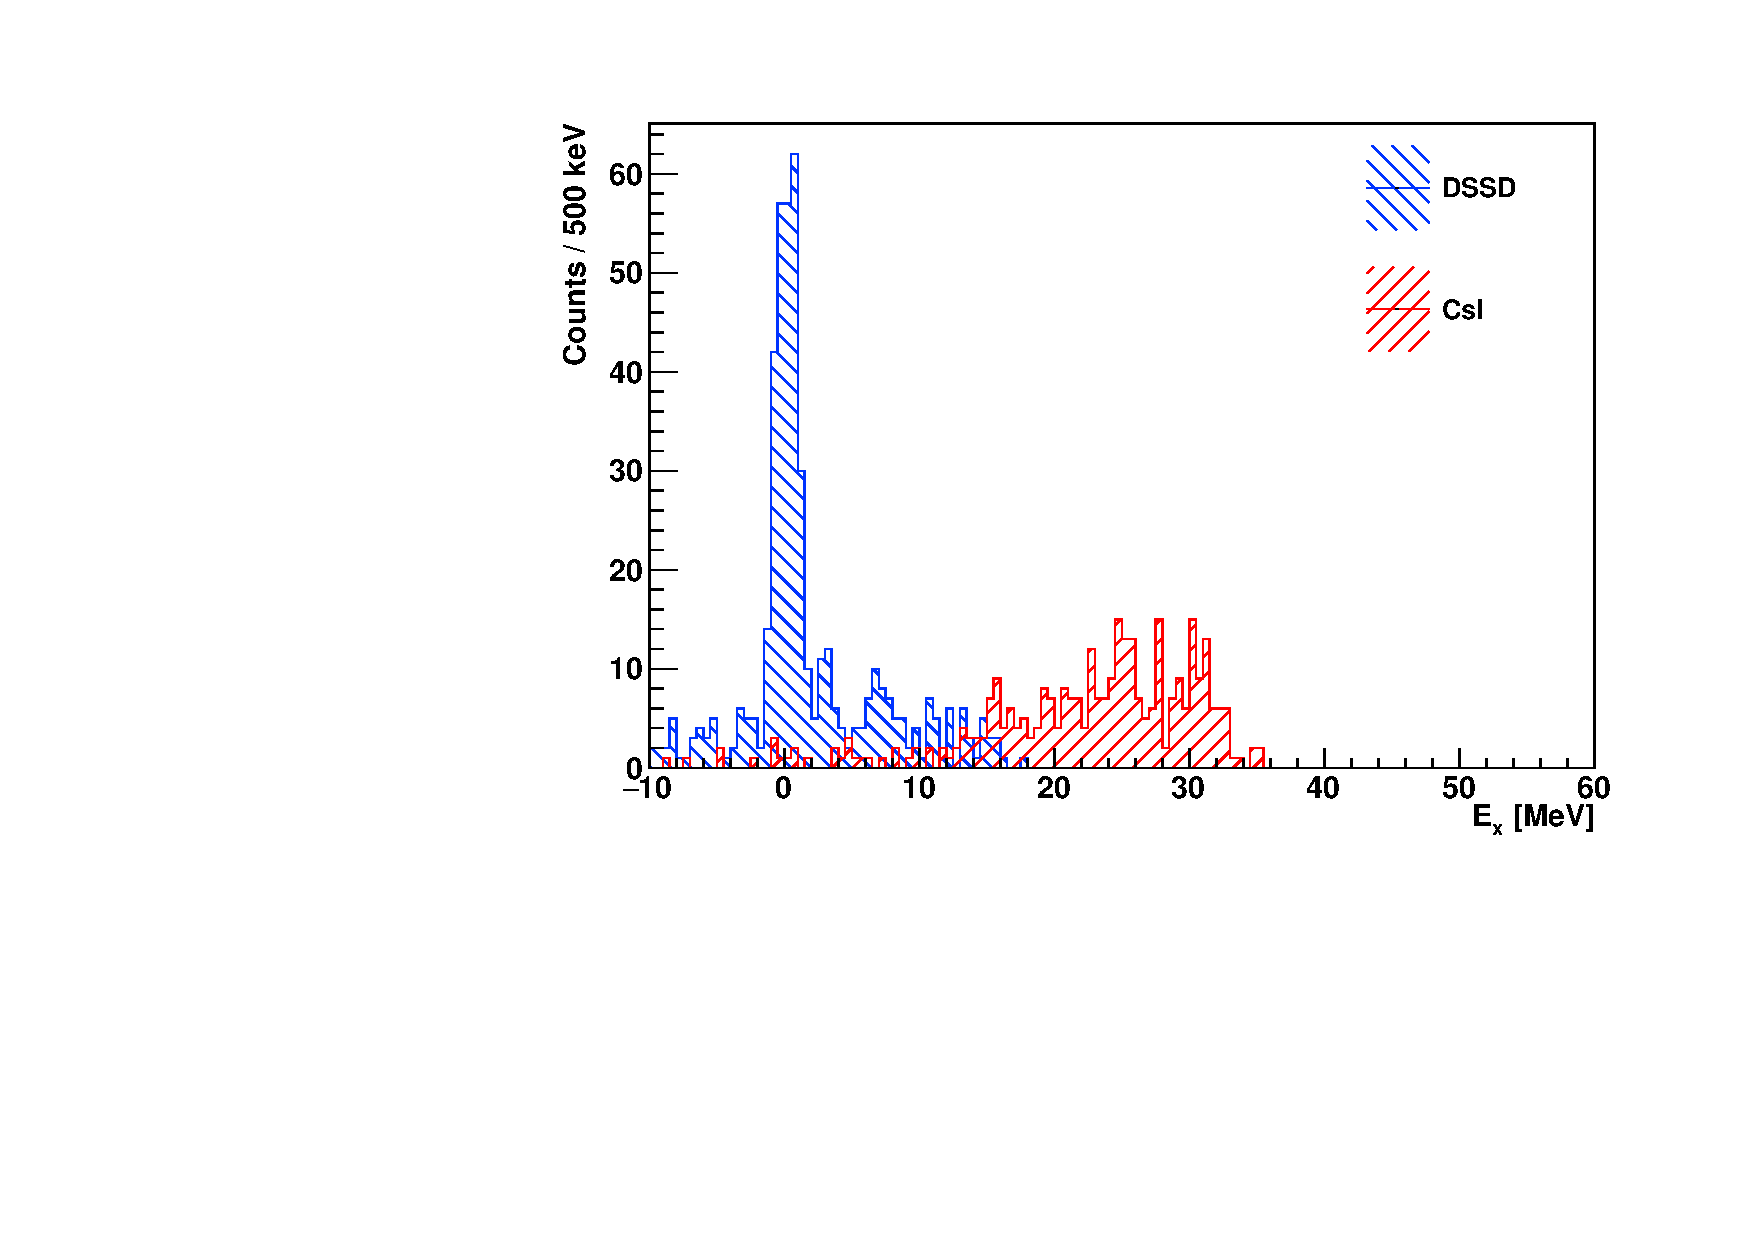
\includegraphics[width=\textwidth]{figures/with_without_csi_9Li.pdf}
        \captionof{figure}{For \iso{10}{Be}(d, \iso{3}{He})\iso{9}{Li}}
    \end{minipage}
\end{frame}

\begin{frame}[t]{Beam ID}
    Using Caviar to CATS1 TOF and energy loss in IC

    \begin{figure}
        \centering
        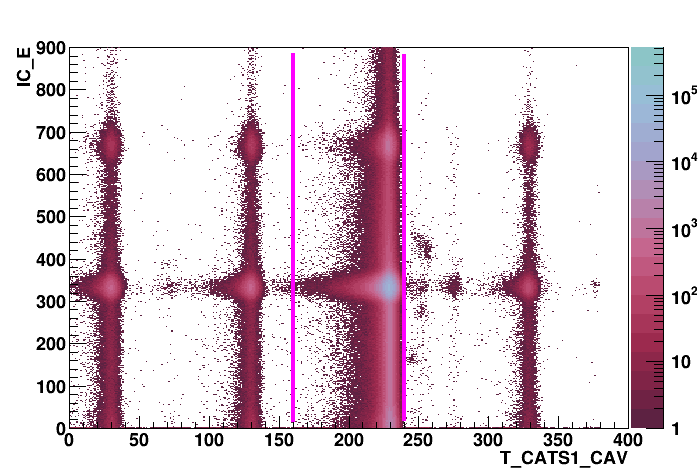
\includegraphics[width=0.7\linewidth]{figures/beam_id_10Be.png}
        \caption{For \iso{10}{Be}}
    \end{figure}
\end{frame}

\begin{frame}[c]{Kinematic lines}
    \begin{minipage}[t]{0.48\linewidth}
        \centering
        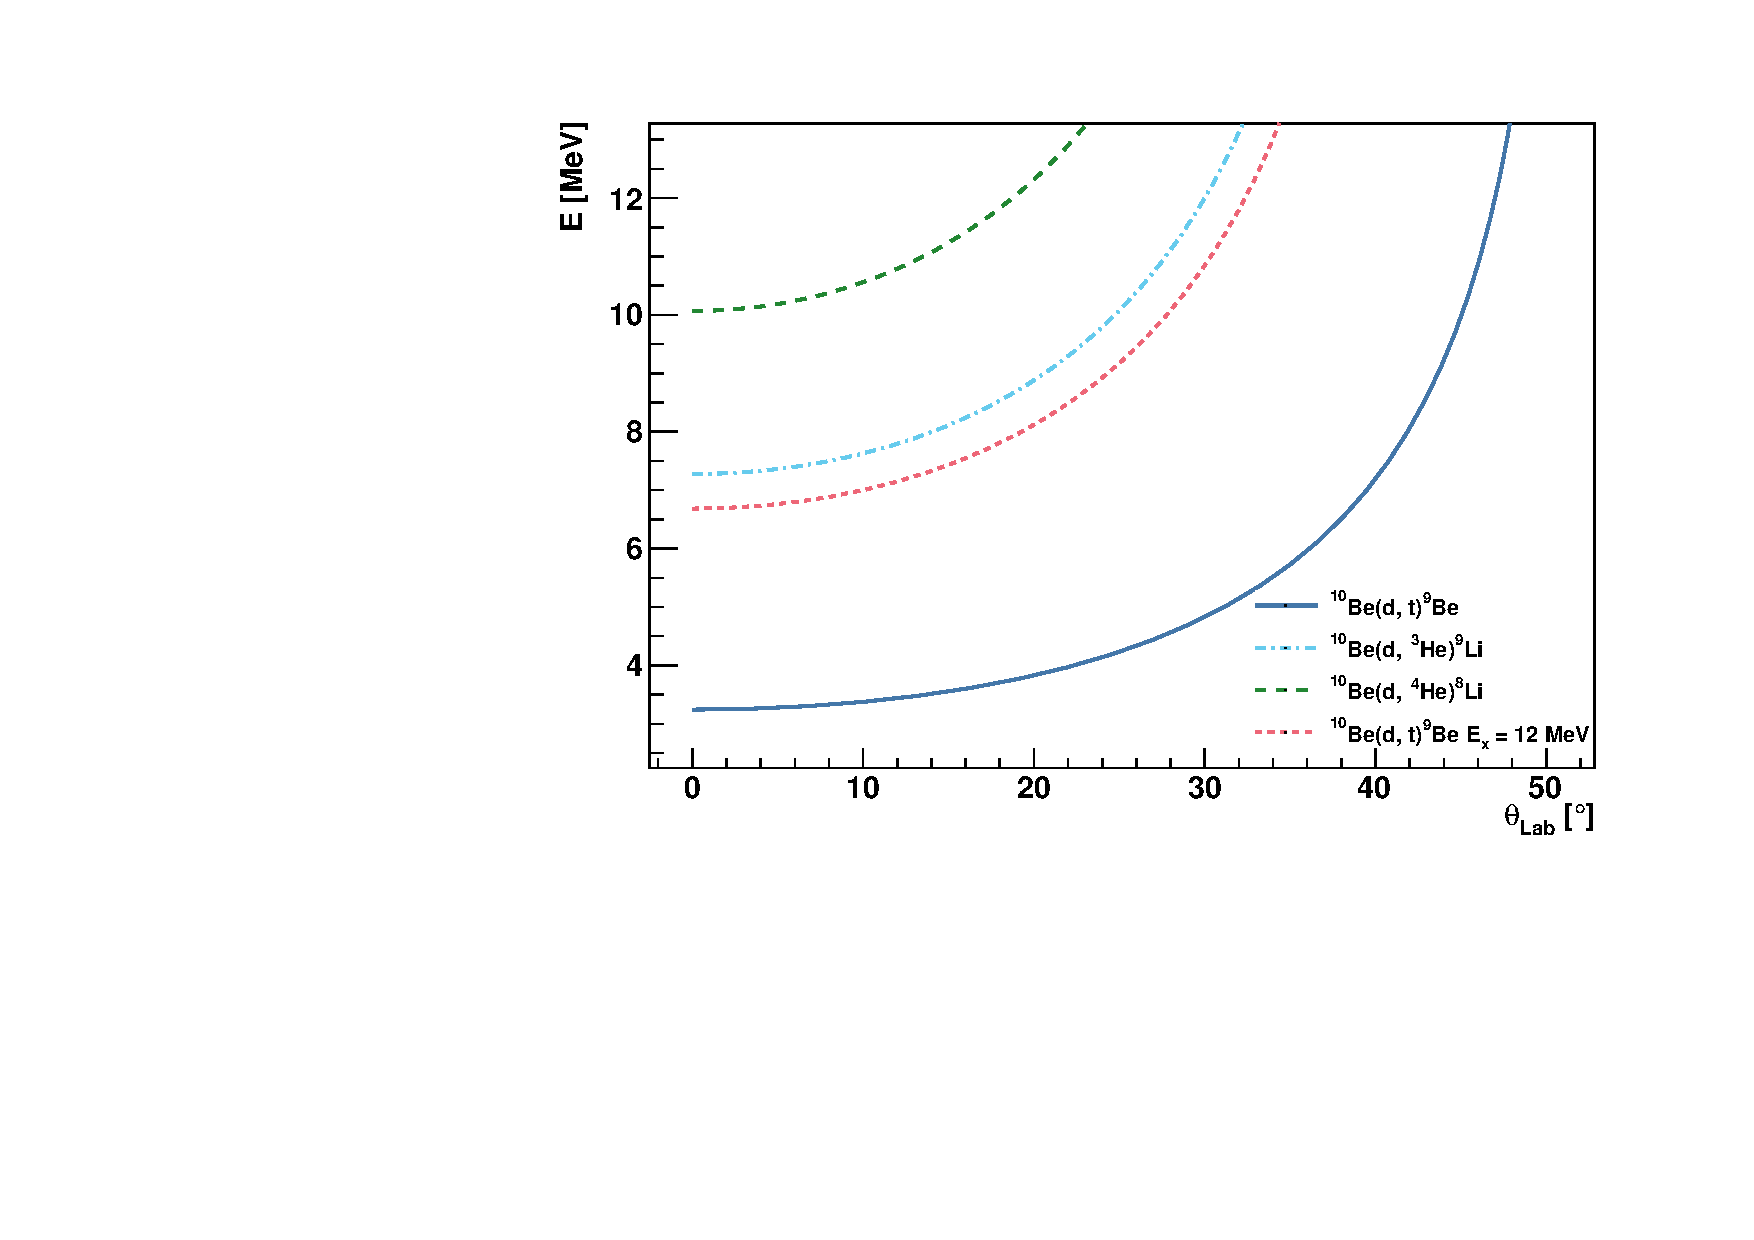
\includegraphics[width=\textwidth]{figures/kinematics_10Be.pdf}
        \captionof{figure}{For \iso{10}{Be} beam}
    \end{minipage}%
    \hfill
    \begin{minipage}[t]{0.48\linewidth}
        \centering
        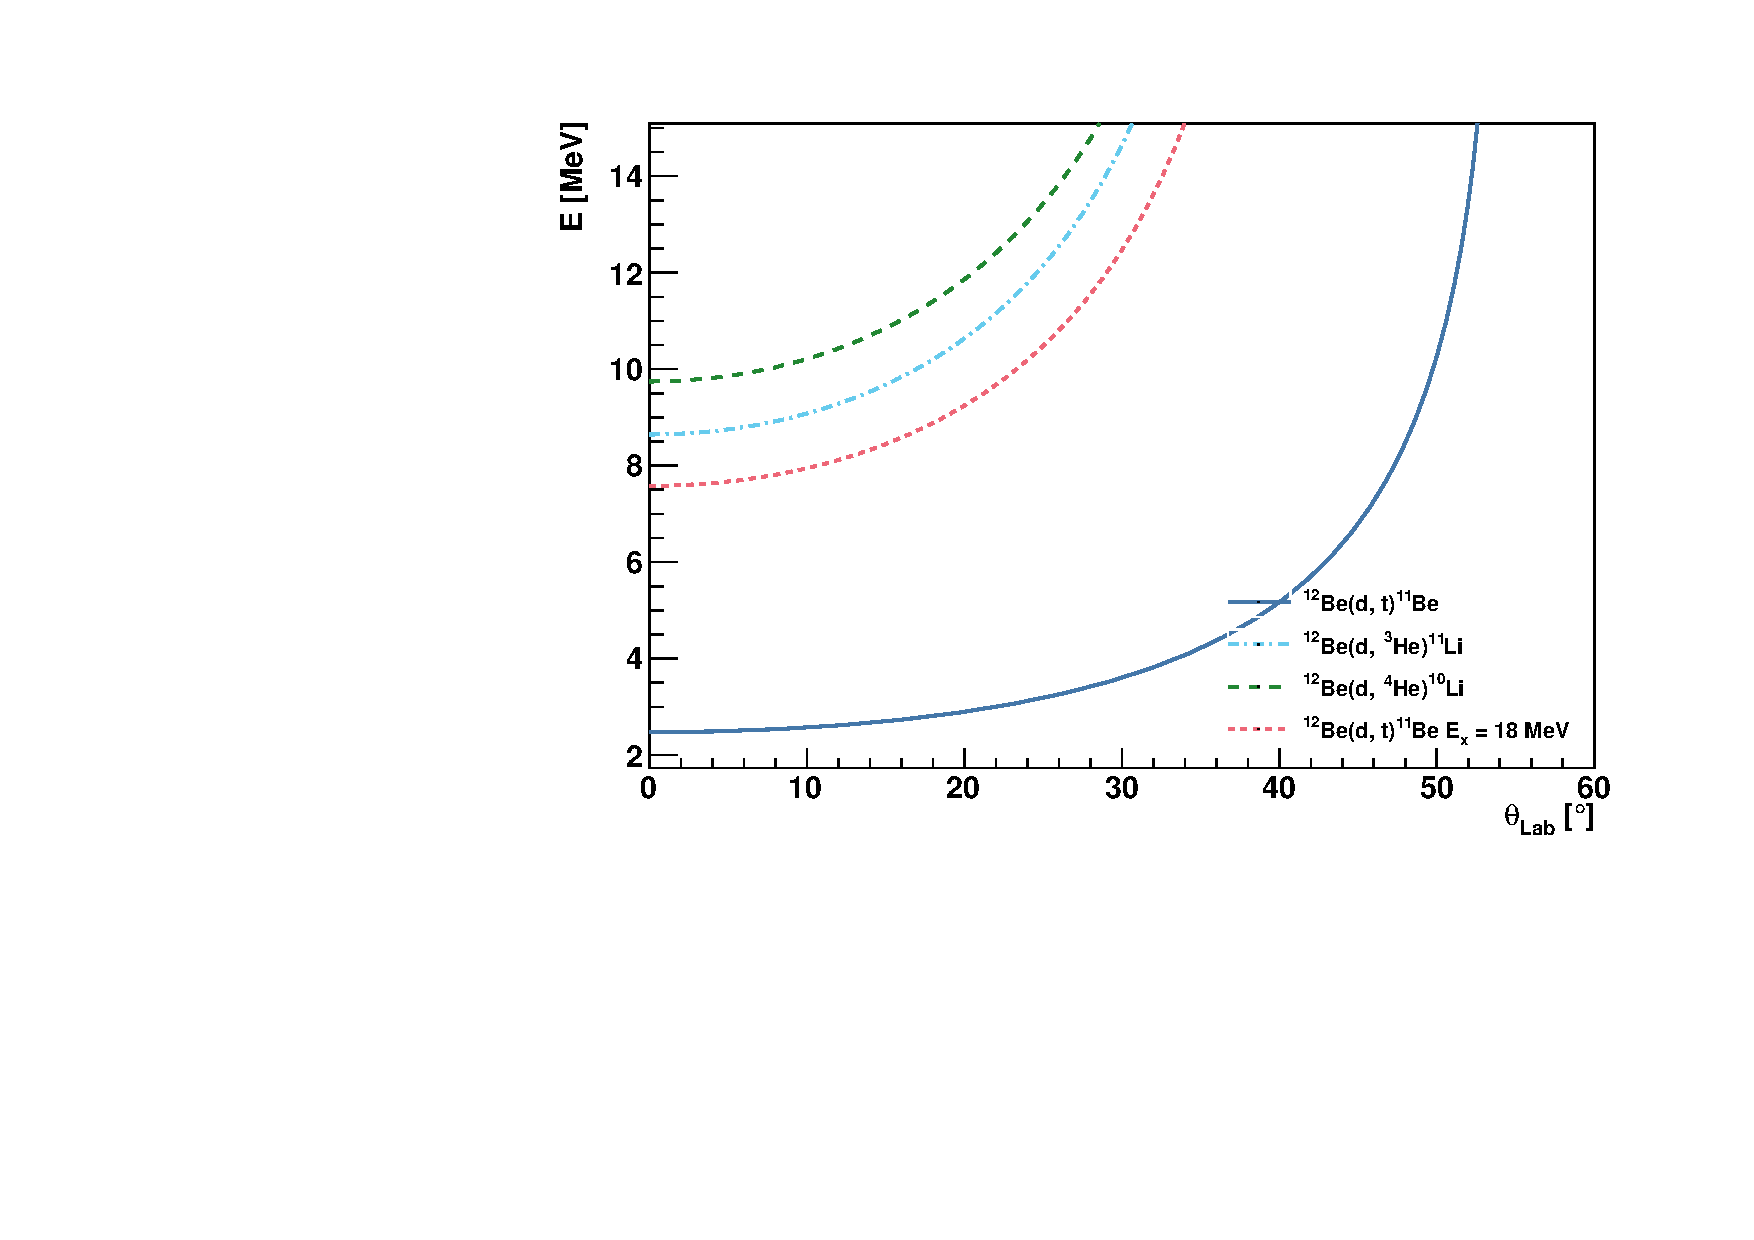
\includegraphics[width=\textwidth]{figures/kinematics_12Be.pdf}
        \captionof{figure}{For \iso{12}{Be} beam}
    \end{minipage}
\end{frame}

\end{document}